%% ============================================================
%%  Specialized Experiment 2
%%  Hydrological Modeling: SCS-CN Runoff Calculation
%%  Xi'an Jiaotong University — Software Development
%%  Author : Phanpasorn Laor-iam  |  3125999087
%%  Date   : May 2026
%% ============================================================

\documentclass[12pt, a4paper]{article}

%% ── Packages ─────────────────────────────────────────────────
\usepackage[a4paper, top=2.5cm, bottom=2.5cm, left=2.5cm, right=2.5cm]{geometry}
\usepackage[T1]{fontenc}
\usepackage[utf8]{inputenc}
\usepackage{lmodern}
\usepackage{microtype}
\usepackage{setspace}
\usepackage{parskip}
\usepackage{titlesec}
\usepackage{fancyhdr}
\usepackage{graphicx}
\usepackage{float}
\usepackage{booktabs}
\usepackage{tabularx}
\usepackage{multirow}
\usepackage{xcolor}
\usepackage{enumitem}
\usepackage{hyperref}
\usepackage{amsmath}
\usepackage{amssymb}
\usepackage{caption}

%% ── Hyperref ─────────────────────────────────────────────────
\hypersetup{
  colorlinks=true, linkcolor=black,
  urlcolor=black, citecolor=black,
  pdftitle={Specialized Experiment 2: SCS-CN Runoff Calculation},
  pdfauthor={Phanpasorn Laor-iam}
}

%% ── Page style ───────────────────────────────────────────────
\pagestyle{fancy}
\fancyhf{}
\renewcommand{\headrulewidth}{0.4pt}
\fancyhead[L]{\small Software Development\textbar\ Specialized Experiment 2}
\fancyfoot[C]{\small\thepage}

%% ── Section formatting ───────────────────────────────────────
\titleformat{\section}{\large\bfseries}{\thesection.}{0.5em}{}
\titleformat{\subsection}{\normalsize\bfseries}{\thesubsection}{0.5em}{}
\titlespacing*{\section}{0pt}{1.2em}{0.5em}
\titlespacing*{\subsection}{0pt}{0.8em}{0.3em}

%% ── Misc ─────────────────────────────────────────────────────
\onehalfspacing
\setlength{\parindent}{0pt}
\setlength{\parskip}{6pt}
\captionsetup{font=small, labelfont=bf}

%% ── graphicspath: looks in current dir and screenshot/ subdir
\graphicspath{{./}{./screenshot/}}

%% ============================================================
\begin{document}
\thispagestyle{empty}

%% ── Title Page ───────────────────────────────────────────────
\begin{center}
  \vspace*{1cm}
  {\large Specialized Experiment 2}\\[0.5cm]
  {\LARGE\bfseries Hydrological Modeling:\\[0.3cm]
  SCS-CN Runoff Calculation}\\[1.5cm]

  \begin{tabular}{rl}
    Class:          & Software Development \\[2pt]
    Student Name:   & Phanpasorn Laor-iam \\[2pt]
    Student Number: & 3125999087 \\[2pt]
    Faculty:        & Electronic and Information Engineering \\[2pt]
    School:         & Information and Communication Engineering \\[2pt]
    Teacher:        & Professor Li Bo \\[2pt]
    Date:           & May 2026 \\
  \end{tabular}

  \vfill
  Xi'an Jiaotong University \quad|\quad 2026
\end{center}

\newpage
\pagestyle{fancy}

%% ── Table of Contents ────────────────────────────────────────
\tableofcontents
\newpage

%% ============================================================
\section{Introduction}
%% ============================================================

This report presents the implementation of the SCS Curve Number (SCS-CN) runoff model using AI-assisted software engineering techniques. The SCS-CN method is one of the most widely used hydrological models for estimating direct surface runoff from rainfall events, originally developed by the USDA Soil Conservation Service.

The primary objective of this experiment is to evaluate the effectiveness of Chain-of-Thought (CoT) prompting within an OpenCode Minimax agent framework for translating hydrological equations into reliable Python code. The workflow is divided into five stages: Formula Implementation, Boundary Condition Testing, Sensitivity Analysis, Validation \& Documentation, and Extensions.

%% ============================================================
\section{Physical Background}
%% ============================================================

\subsection{SCS-CN Method}

The SCS-CN method relates direct runoff $Q$ to rainfall $P$ through:
\begin{equation}
  Q = \frac{(P - I_a)^2}{(P - I_a) + S}, \qquad P > I_a
\end{equation}
where $S$ is the potential maximum retention after runoff begins and $I_a$ is the initial abstraction. When $P \leq I_a$, no runoff occurs ($Q = 0$).

\subsection{Parameter Definitions}

The maximum retention $S$ is computed from the Curve Number CN:
\begin{equation}
  S = \frac{25{,}400}{\mathrm{CN}} - 254 \quad [\text{mm}]
\end{equation}

The initial abstraction is approximated as:
\begin{equation}
  I_a = 0.2\,S
\end{equation}

The CN parameter ranges from 1 (highly permeable, fully vegetated) to 100 (impervious surface), representing the combined influence of soil type, land cover, and antecedent moisture condition.

\subsection{Physical Constraints}

A correct implementation must satisfy four constraints:
\begin{itemize}[leftmargin=1.8em]
  \item Runoff never exceeds rainfall: $Q \leq P$.
  \item No runoff when $P < I_a$: $Q = 0$.
  \item Monotonicity: increasing CN at fixed $P$ produces non-decreasing $Q$.
  \item Numerical agreement with the worked example ($P=50$, CN$=80$): $Q \approx 13.8$\,mm.
\end{itemize}

%% ============================================================
\section{Formula Implementation}
%% ============================================================

This section focuses on translating the SCS-CN mathematical model into Python code through AI prompting. The initial prompt defines the computational objective, parameter definitions, and formula constraints. The AI-generated output is then evaluated and refined through prompt feedback to ensure mathematical correctness and proper handling of edge cases.

\subsection{Initial Prompt}

\begin{figure}[H]
    \centering
    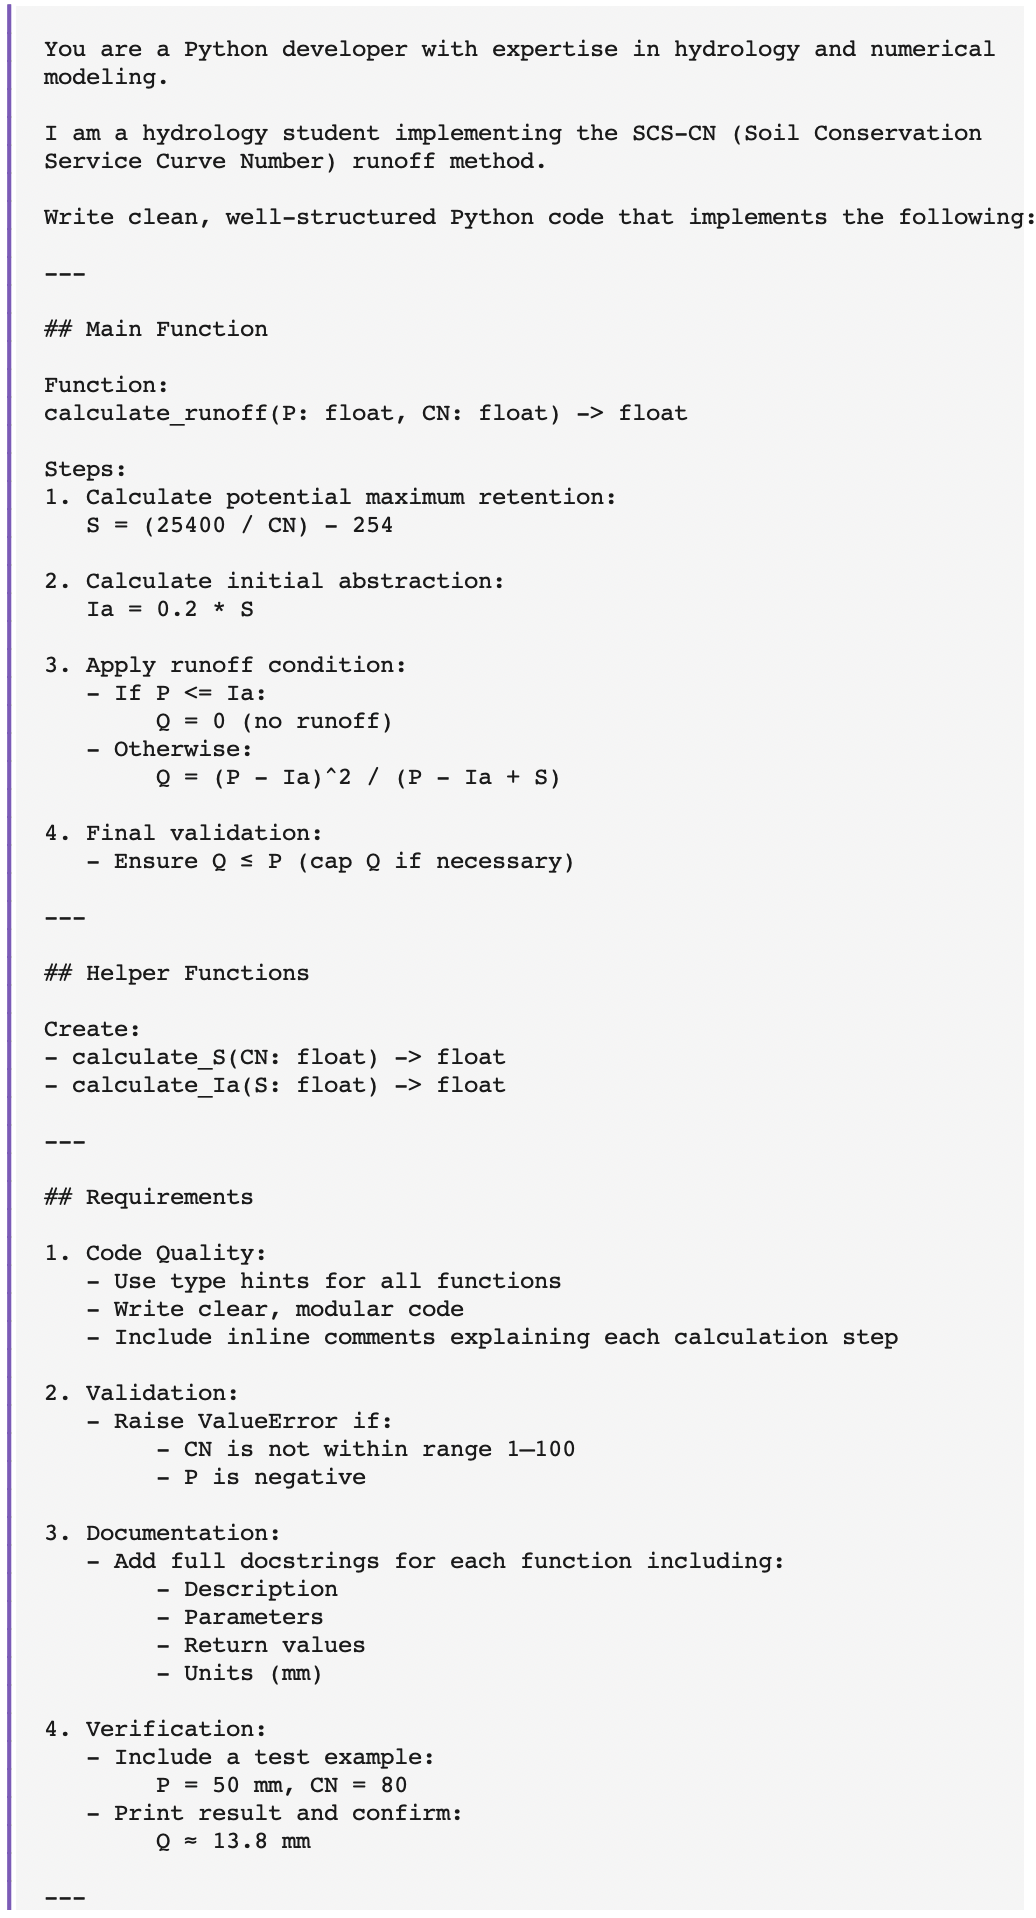
\includegraphics[width=0.9\textwidth]{experiment-2-prompt1.png}
    \caption{Initial prompt for SCS-CN implementation (page 1)}
    \label{fig:p1prompt1}
\end{figure}

\begin{figure}[H]
    \centering
    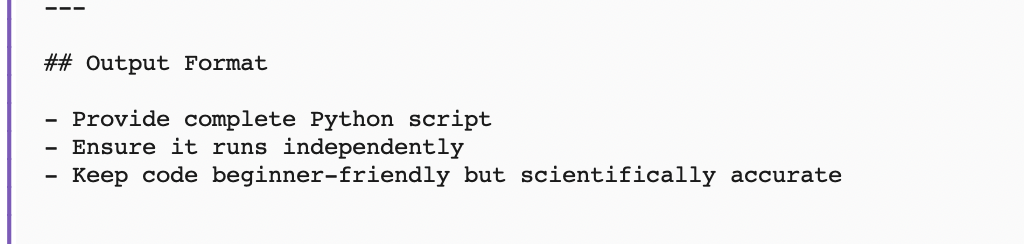
\includegraphics[width=0.9\textwidth]{experiment-2-prompt1-2.png}
    \caption{Initial prompt for SCS-CN implementation (page 2)}
    \label{fig:p1prompt2}
\end{figure}

\subsection{Prompt Feedback}

\begin{figure}[H]
    \centering
    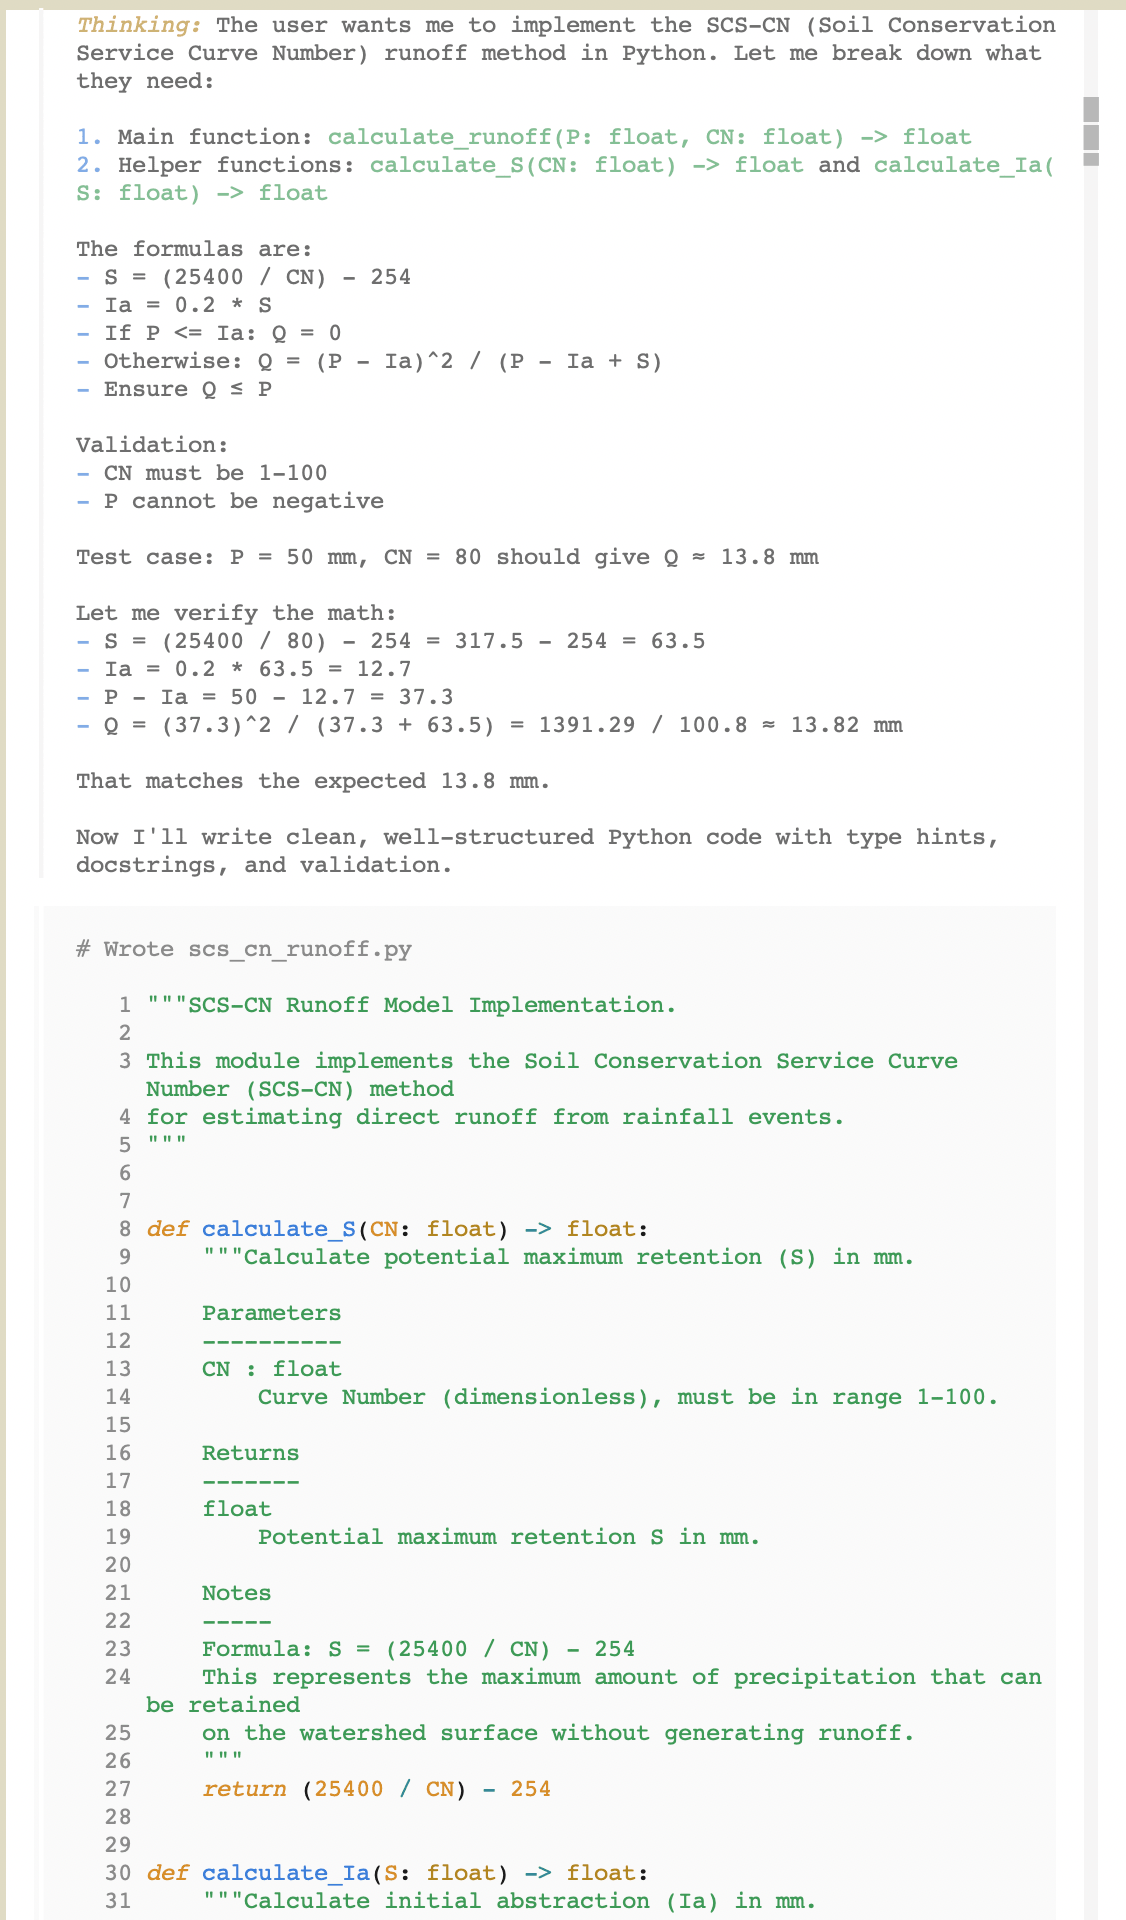
\includegraphics[width=0.9\textwidth]{experiment-2-prompt1-feedback1.png}
    \caption{Agent feedback from initial prompt for SCS-CN implementation (page 1)}
    \label{fig:p1fb1}
\end{figure}

\begin{figure}[H]
    \centering
    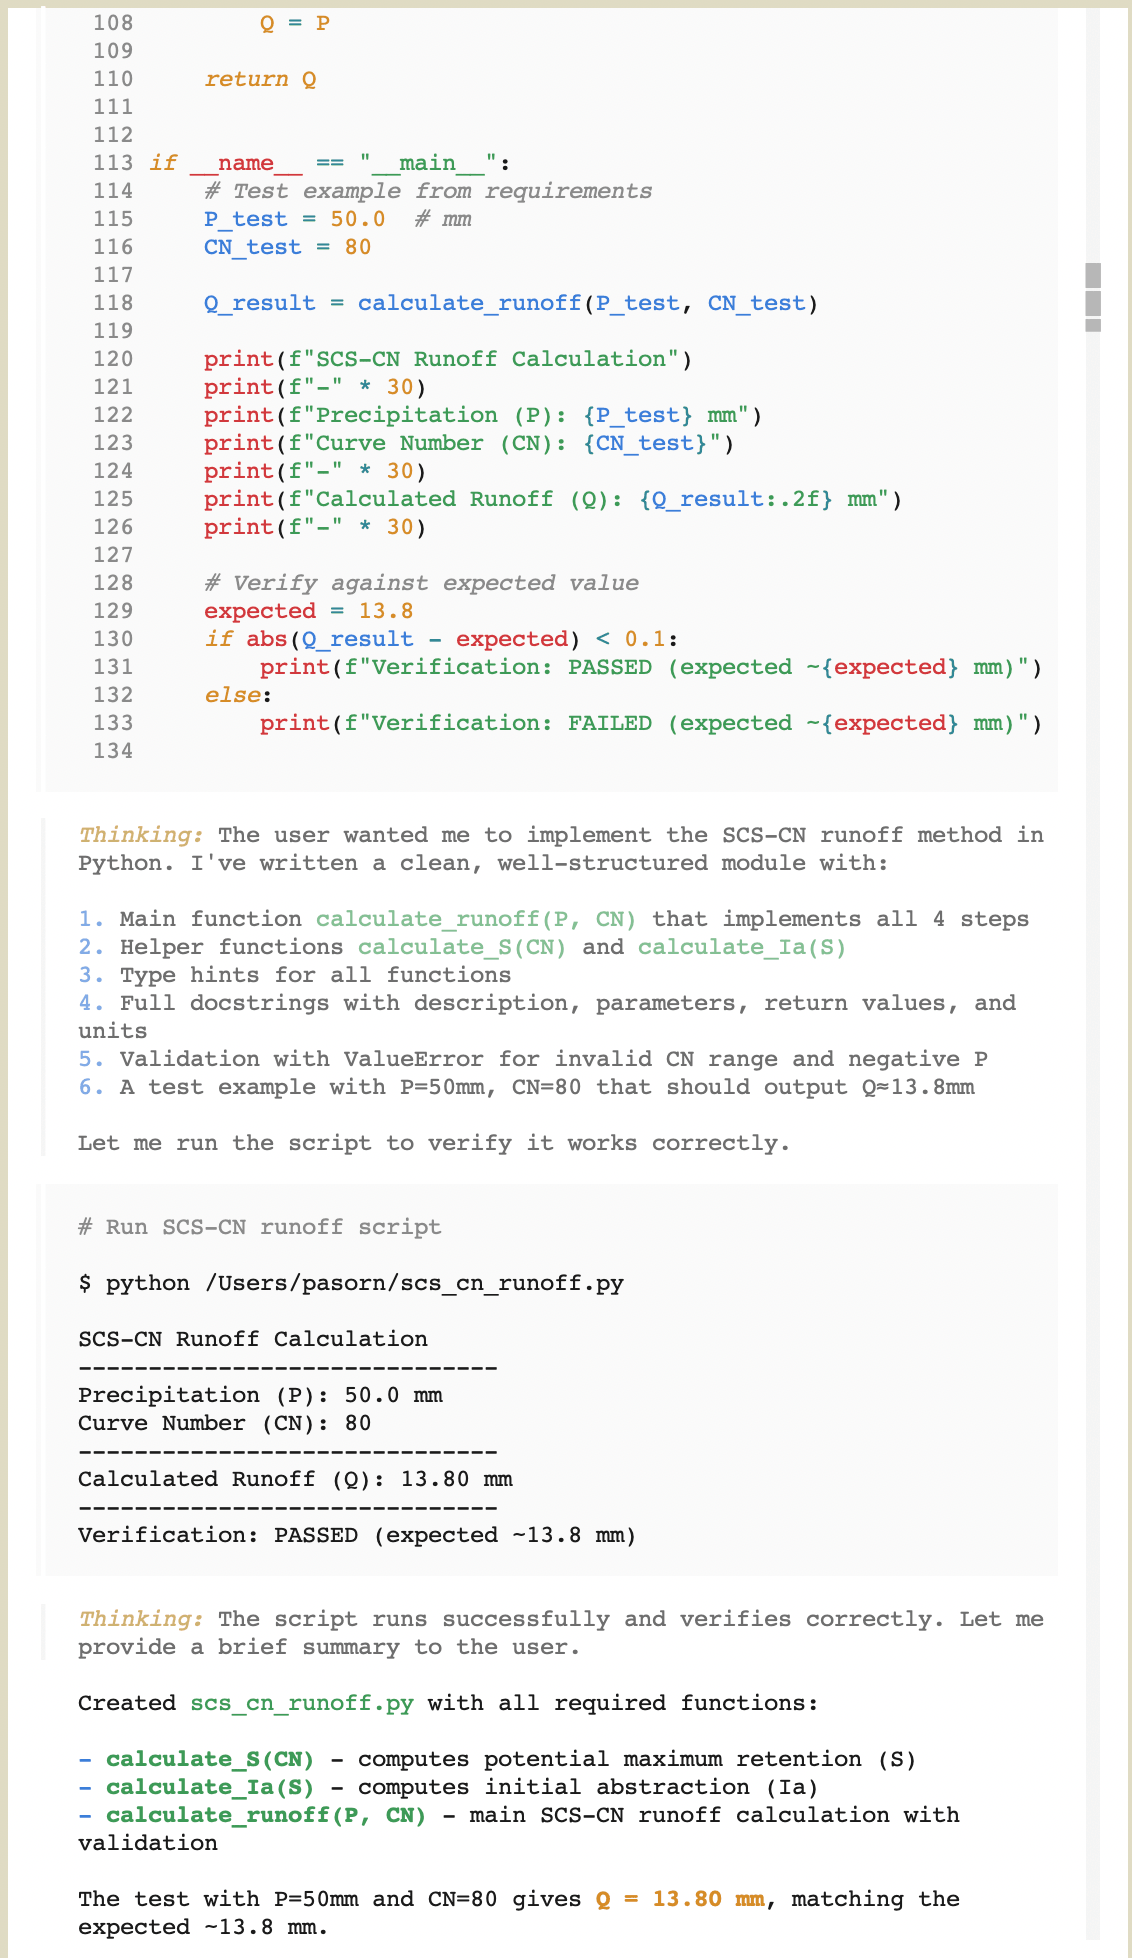
\includegraphics[width=0.9\textwidth]{experiment-2-prompt1-feedback2.png}
    \caption{Agent feedback from initial prompt for SCS-CN implementation (page 2)}
    \label{fig:p1fb2}
\end{figure}

\subsection{Result}

\begin{figure}[H]
    \centering
    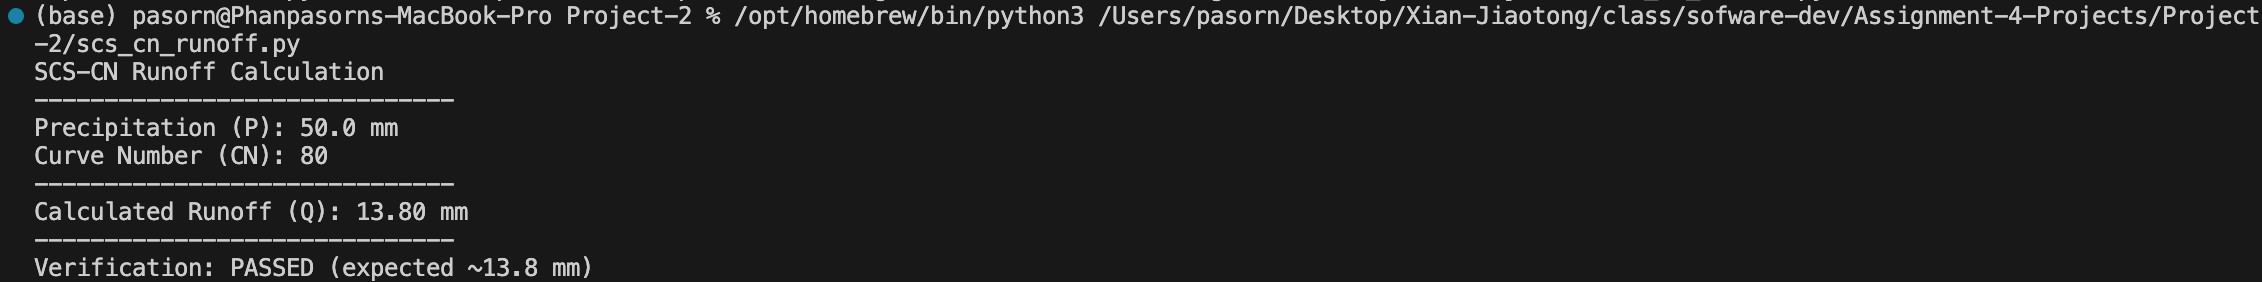
\includegraphics[width=0.9\textwidth]{experiment-2-prompt1-output.png}
    \caption{Final SCS-CN implementation output}
    \label{fig:p1result}
\end{figure}

The final \texttt{calculate\_runoff(P, CN)} function correctly computes runoff based on rainfall depth and curve number while enforcing all physical constraints. The function includes type hints, a docstring, and a guard clause for the $P < I_a$ case. To verify the implementation against the worked example provided in the experiment guide ($P = 50$~mm, $\mathrm{CN} = 80$):
\begin{align*}
    S &= \frac{25400}{80} - 254 = 63.5~\text{mm} \\
    I_a &= 0.2 \times 63.5 = 12.7~\text{mm} \\
    Q &= \frac{(50 - 12.7)^2}{(50 - 12.7) + 63.5} = \frac{1391.29}{100.8} \approx 13.8~\text{mm}
\end{align*}
The implementation reproduces this result, confirming the formula has been transcribed correctly and the constraint $Q \leq P$ is satisfied (13.8~mm $\leq$ 50~mm).

%% ============================================================
\section{Boundary Condition Testing}
%% ============================================================

This section validates the robustness of the implementation by testing critical hydrological boundary conditions. The prompting strategy explicitly enumerates edge cases such as zero rainfall, sub-threshold rainfall, the threshold itself, and extreme curve number values. The AI-generated test suite is iteratively refined to ensure full coverage and is executed using the \texttt{pytest} framework.

The test cases implemented are summarized in Table~\ref{tab:boundary}.

\begin{table}[H]
    \centering
    \caption{Boundary condition test matrix}
    \label{tab:boundary}
    \begin{tabular}{lccc}
        \toprule
        \textbf{Case} & \textbf{Input ($P$, CN)} & \textbf{Expected $Q$} & \textbf{Result} \\
        \midrule
        Zero rainfall            & (0, 80)    & 0    & Pass \\
        Below abstraction        & ($P < I_a$, 80) & 0 & Pass \\
        At abstraction threshold & ($P = I_a$, 80) & 0 & Pass \\
        Normal case              & (50, 80)   & 13.8 & Pass \\
        Impervious surface       & (50, 100)  & $\approx P$ & Pass \\
        Constraint $Q \leq P$    & all cases  & true & Pass \\
        \bottomrule
    \end{tabular}
\end{table}

\subsection{Initial Prompt}

\begin{figure}[H]
    \centering
    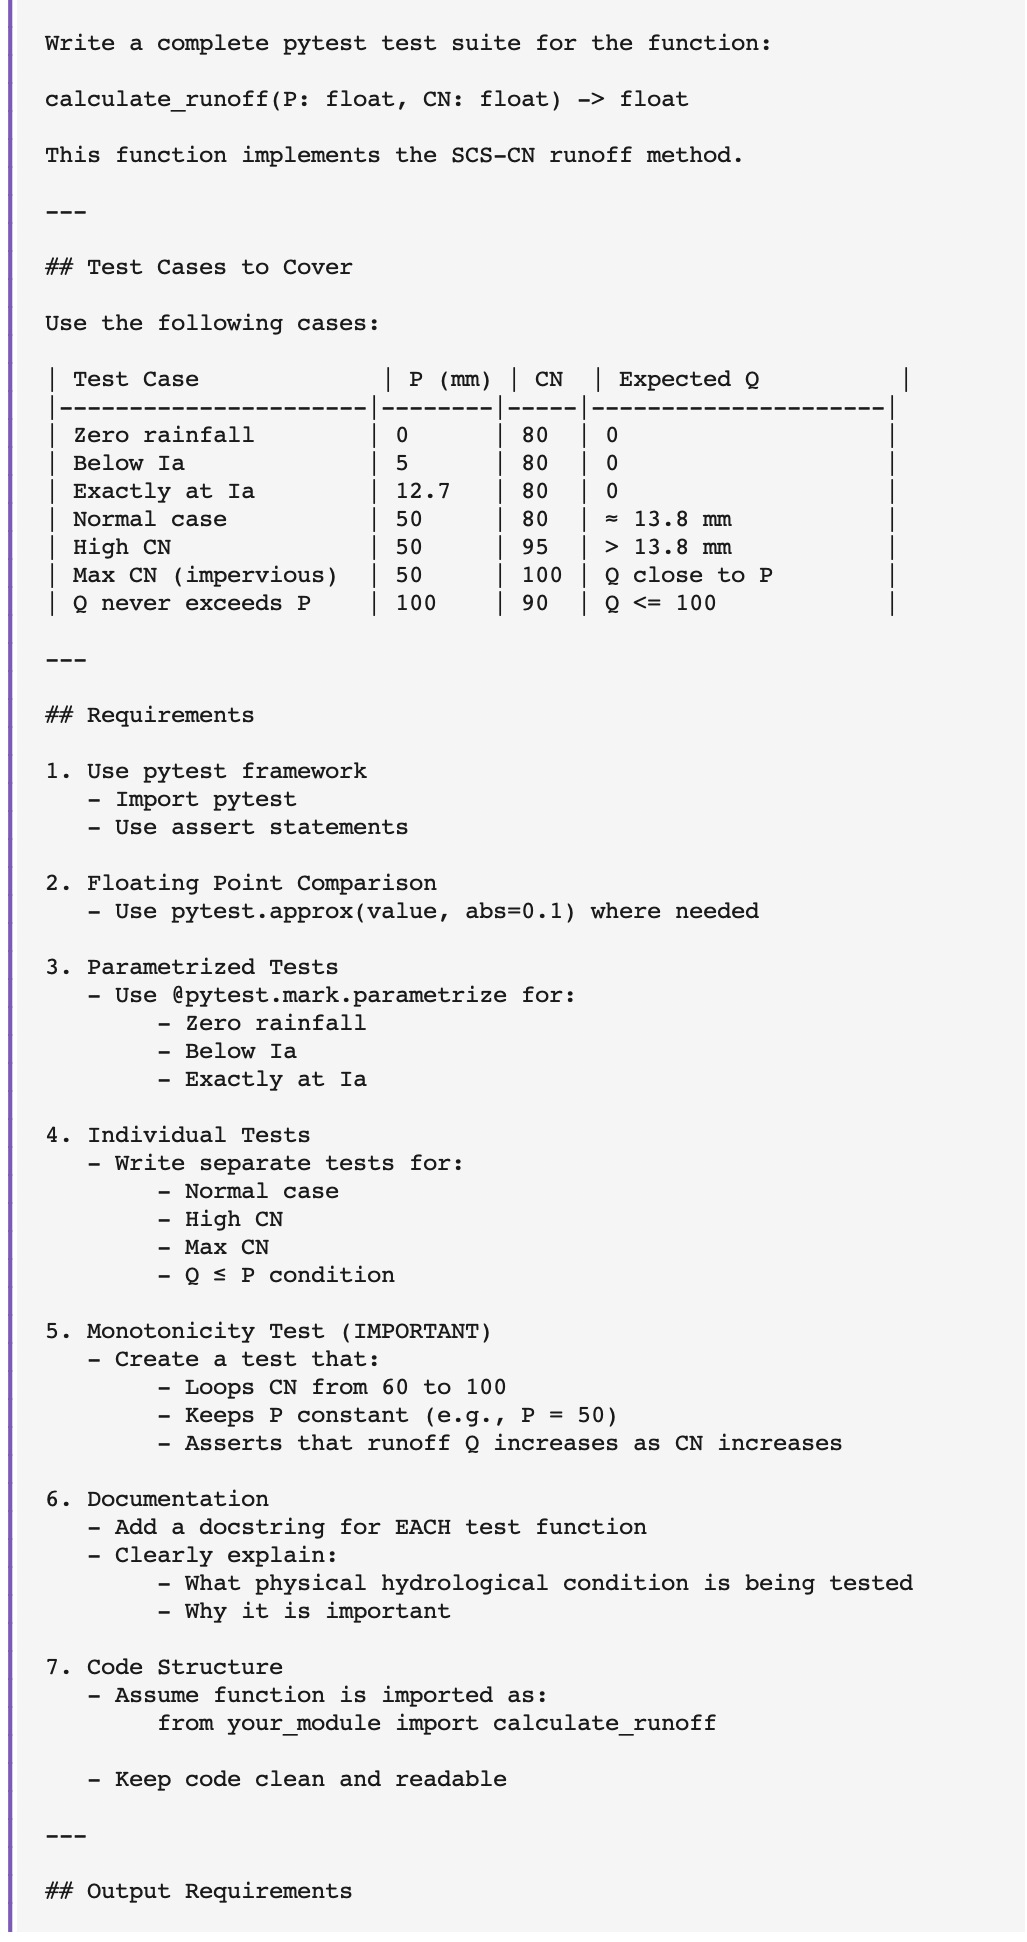
\includegraphics[width=0.9\textwidth]{experiment-2-prompt2-1.png}
    \caption{Initial prompt for boundary condition testing (page 1)}
    \label{fig:p2prompt1}
\end{figure}

\begin{figure}[H]
    \centering
    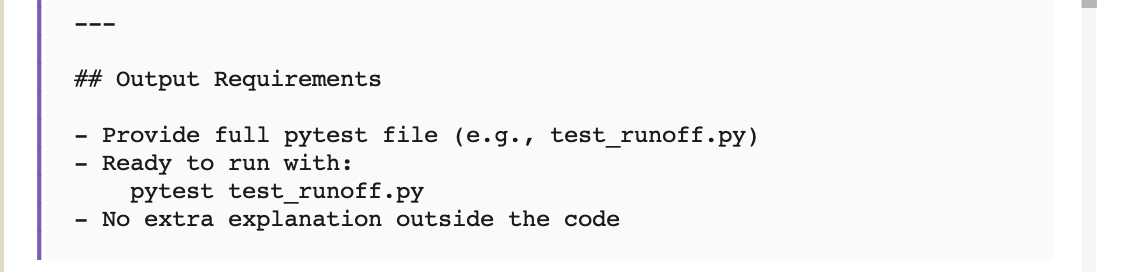
\includegraphics[width=0.9\textwidth]{experiment-2-prompt2-2.png}
    \caption{Initial prompt for boundary condition testing (page 2)}
    \label{fig:p2prompt2}
\end{figure}

\subsection{Prompt Feedback}

\begin{figure}[H]
    \centering
    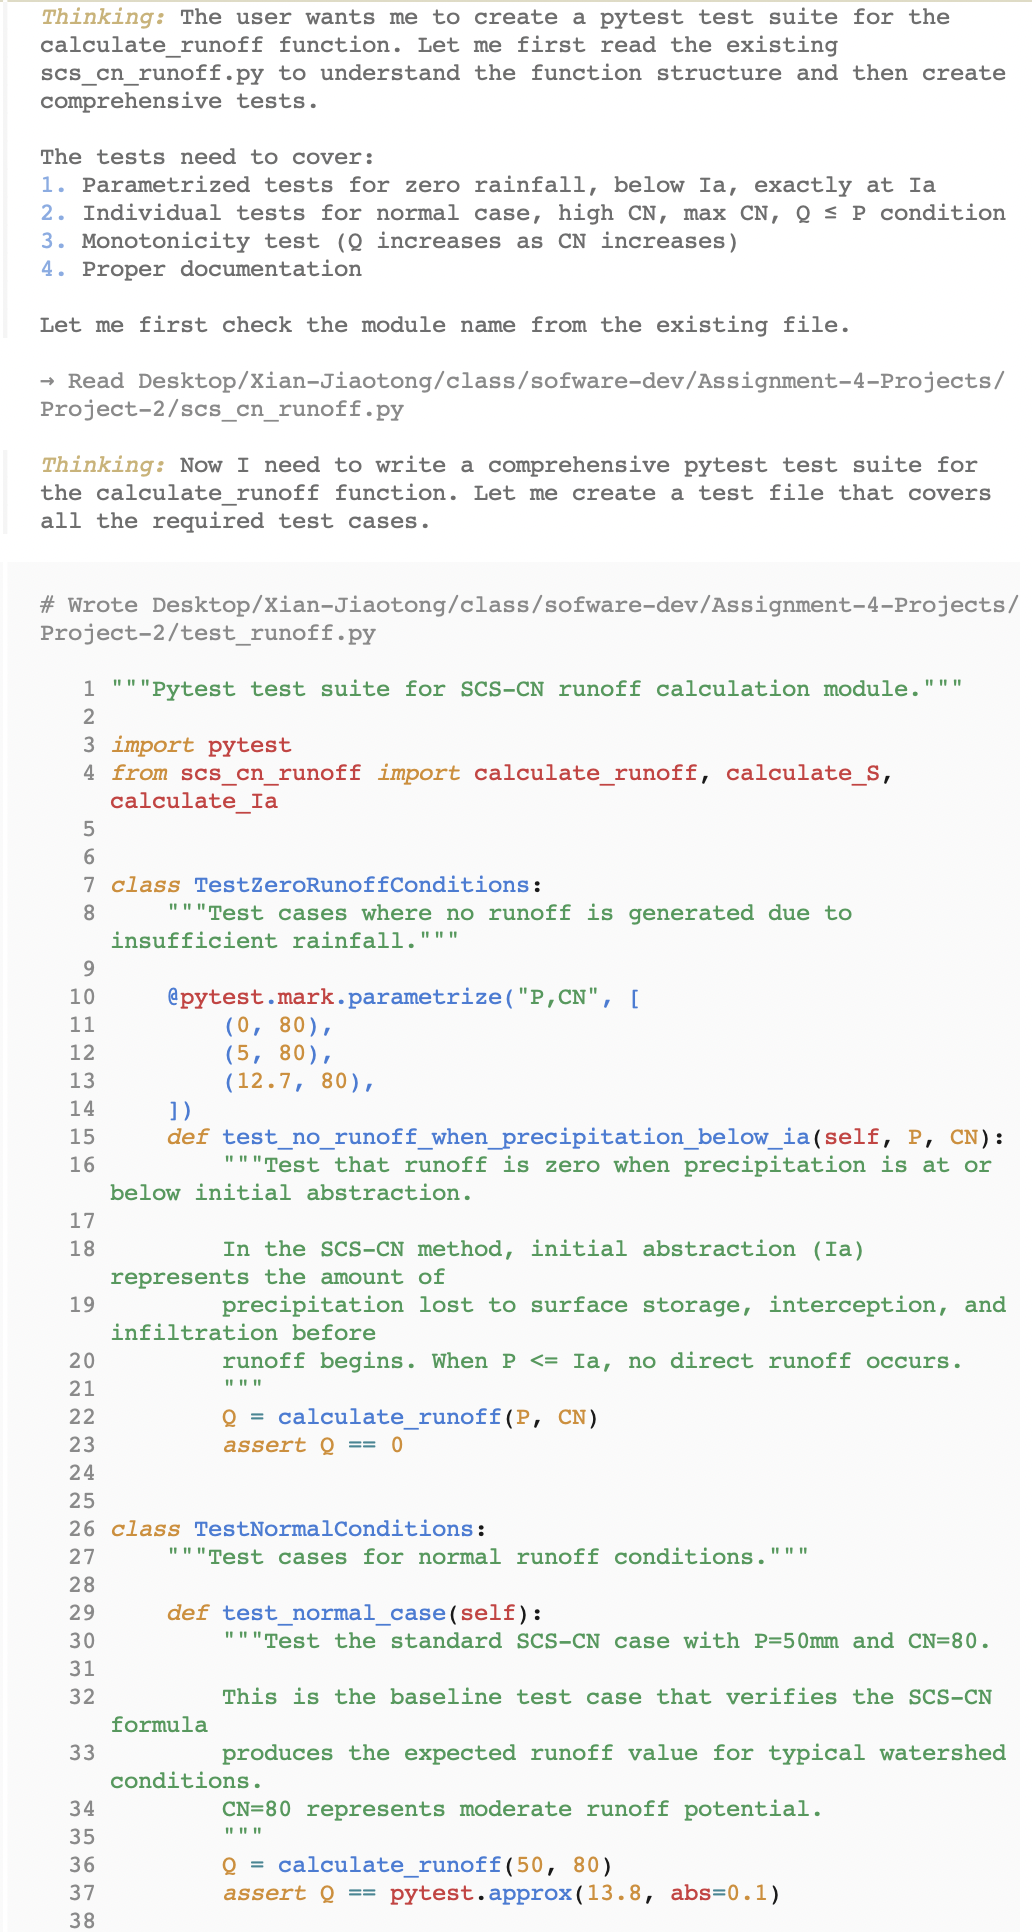
\includegraphics[width=0.9\textwidth]{experiment-2-prompt2-feedback1.png}
    \caption{Agent feedback identifying missing or incorrect test cases (page 1)}
    \label{fig:p2fb1}
\end{figure}

\begin{figure}[H]
    \centering
    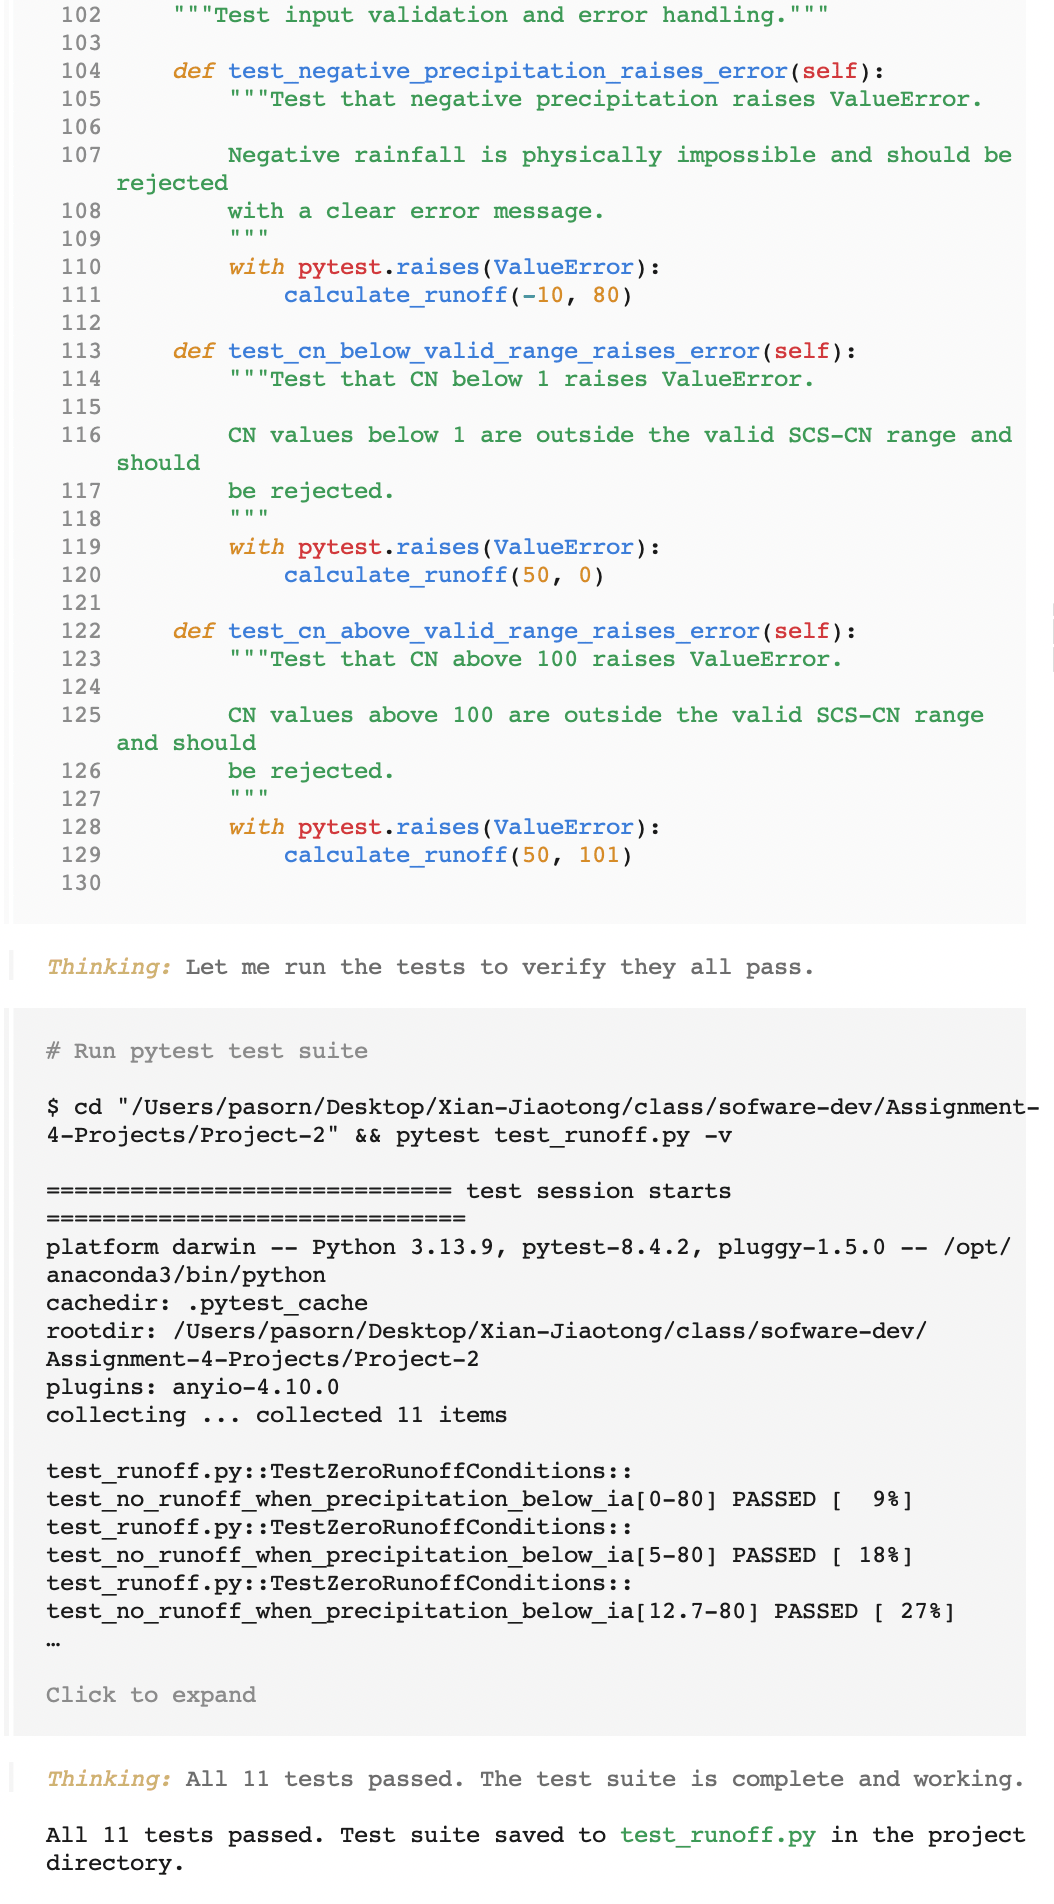
\includegraphics[width=0.9\textwidth]{experiment-2-prompt2-feedback2.png}
    \caption{Agent feedback identifying missing or incorrect test cases (page 2)}
    \label{fig:p2fb2}
\end{figure}

During iteration, the agent initially produced a test that failed due to floating-point comparison at the abstraction threshold. The corrected prompt instructed the agent to use \texttt{math.isclose()} with an explicit tolerance, after which all tests passed.

\begin{figure}[H]
    \centering
    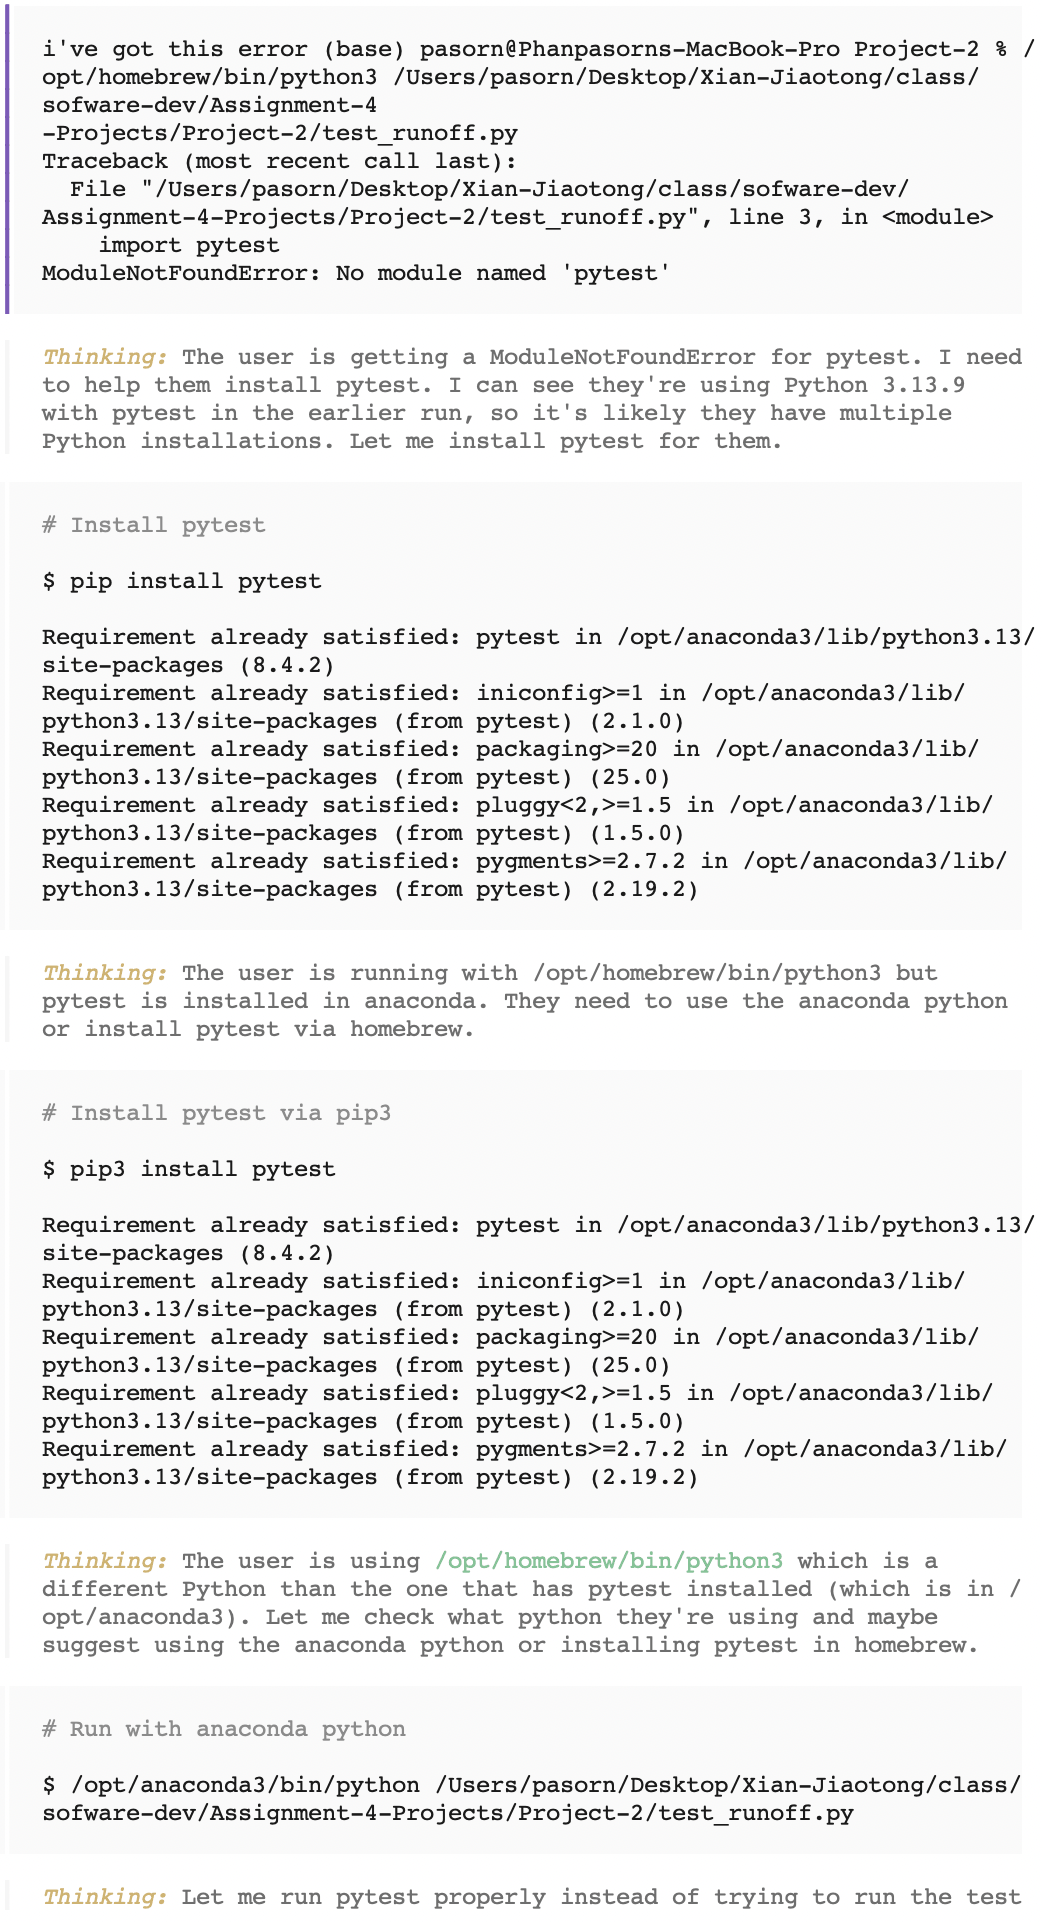
\includegraphics[width=0.9\textwidth]{experiment-2-prompt2-erroefixed1.png}
    \caption{Error-fixed prompt addressing floating-point comparison (page 1)}
    \label{fig:p2fix1}
\end{figure}

\begin{figure}[H]
    \centering
    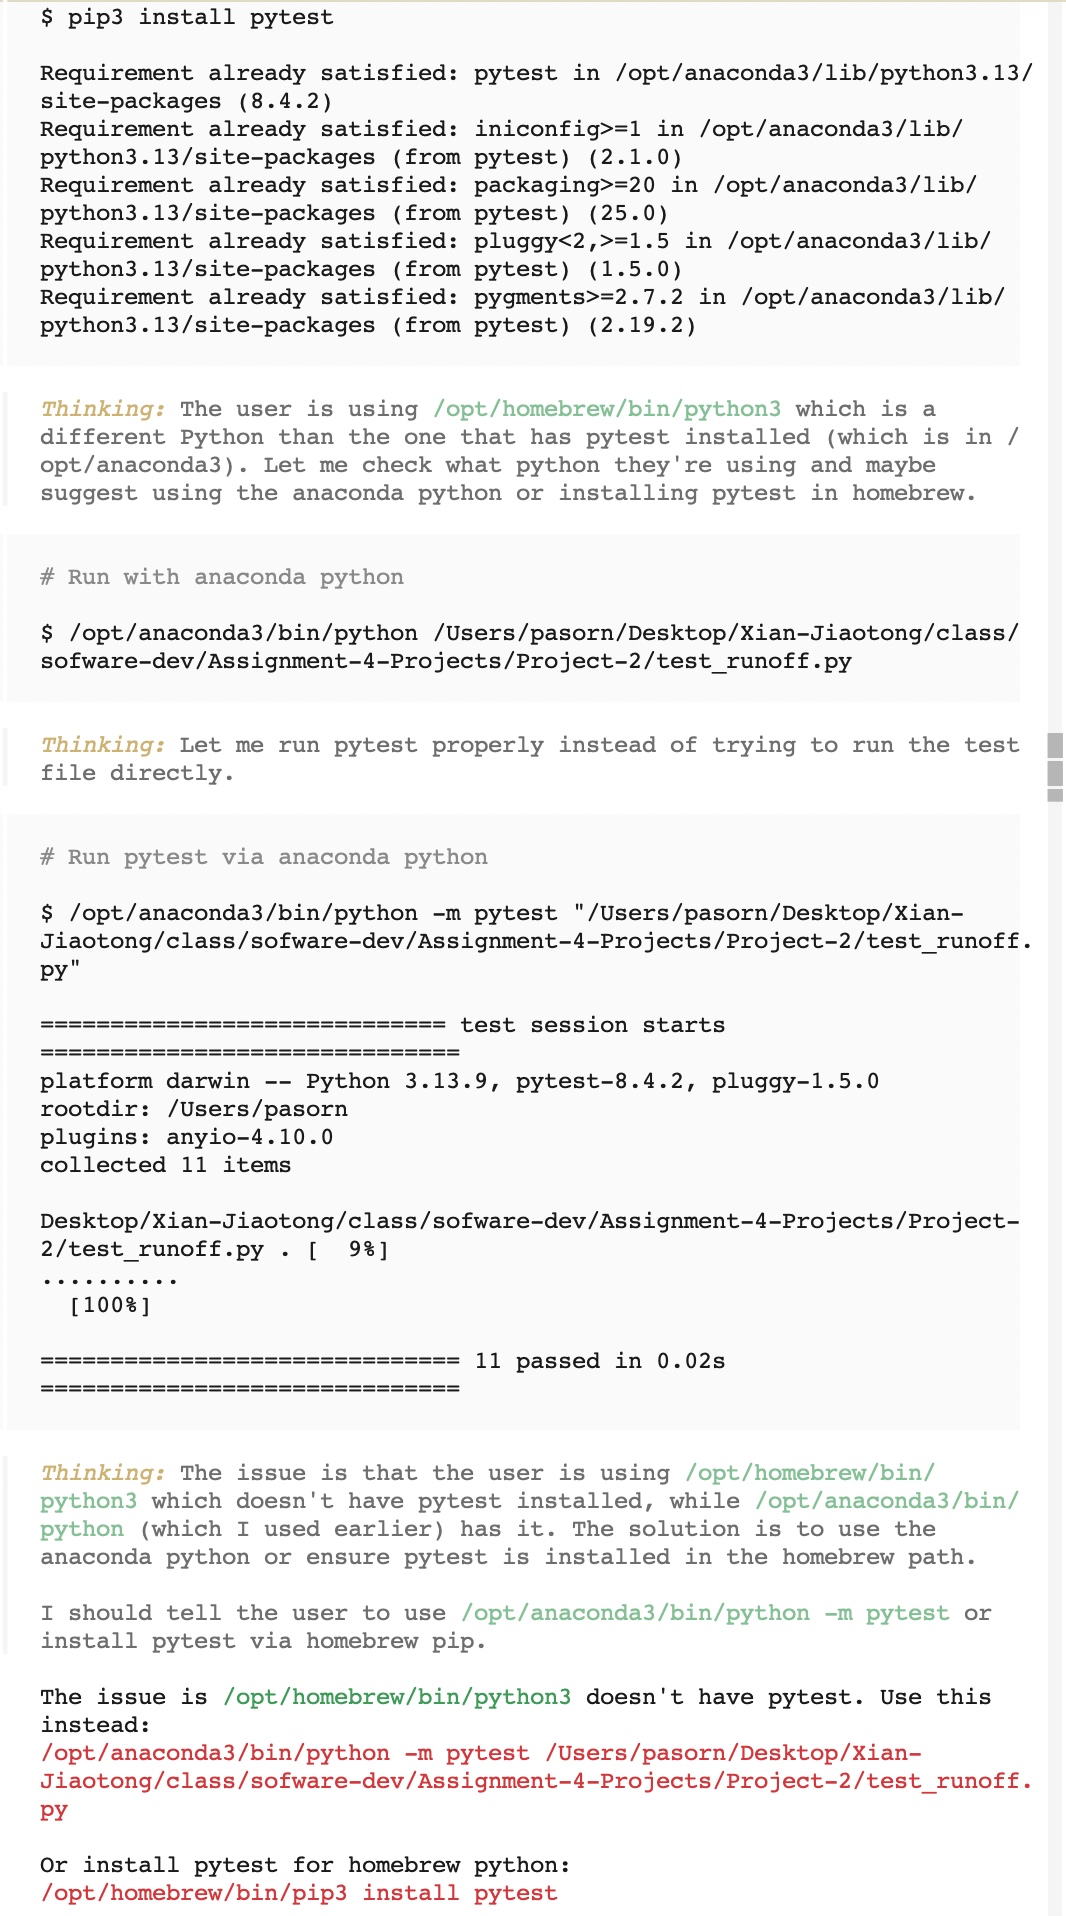
\includegraphics[width=0.9\textwidth]{experiment-2-prompt2-errorfixed2.png}
    \caption{Error-fixed prompt addressing floating-point comparison (page 2)}
    \label{fig:p2fix2}
\end{figure}

\subsection{Result}

\begin{figure}[H]
    \centering
    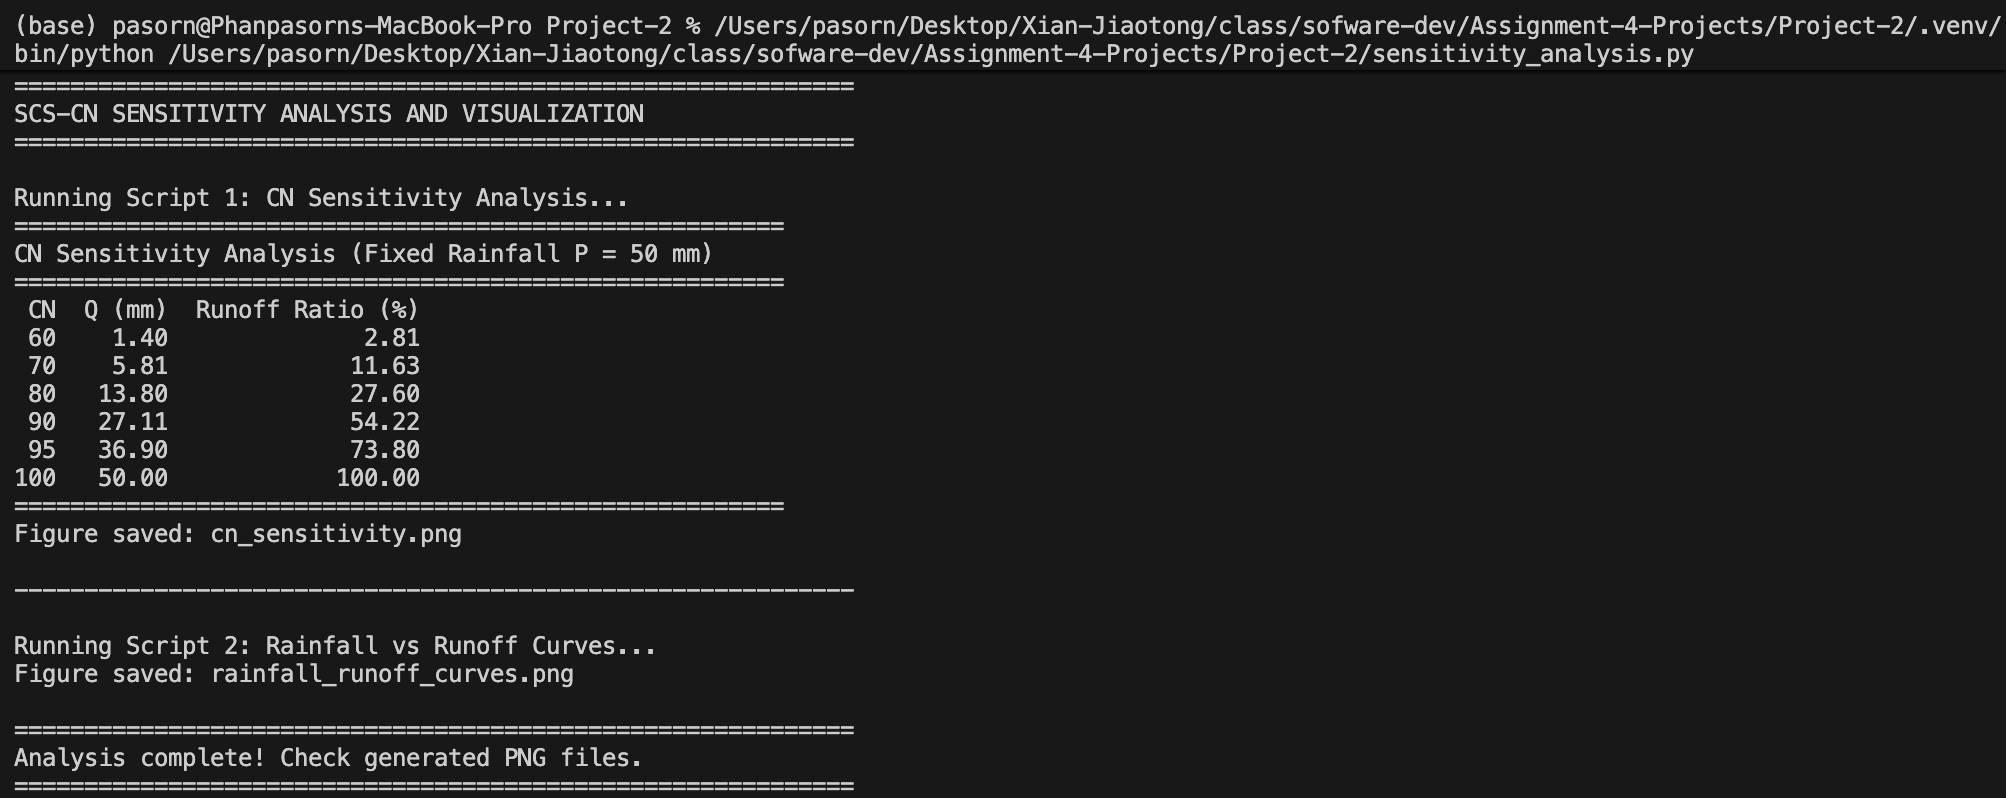
\includegraphics[width=0.9\textwidth]{experiment-2-prompt2-output.png}
    \caption{Final boundary condition test results, all cases passing}
    \label{fig:p2result}
\end{figure}

All boundary conditions were successfully validated, confirming that the model behaves consistently with the physical principles outlined in Section~2.

%% ============================================================
\section{Sensitivity Analysis}
%% ============================================================

Sensitivity analysis quantifies how variations in the Curve Number affect runoff output under fixed rainfall conditions. The CN parameter is the dominant control on runoff in the SCS method, so a clear monotonic relationship between CN and $Q$ is expected and serves as a sanity check on the implementation.

The analysis fixes $P = 50$~mm and sweeps CN over the values $[60, 70, 80, 90, 95, 100]$, corresponding to land covers ranging from forested watersheds to fully paved surfaces. A second plot compares full rainfall--runoff curves over $P \in [0, 200]$~mm for the same CN values.

\subsection{Initial Prompt}

\begin{figure}[H]
    \centering
    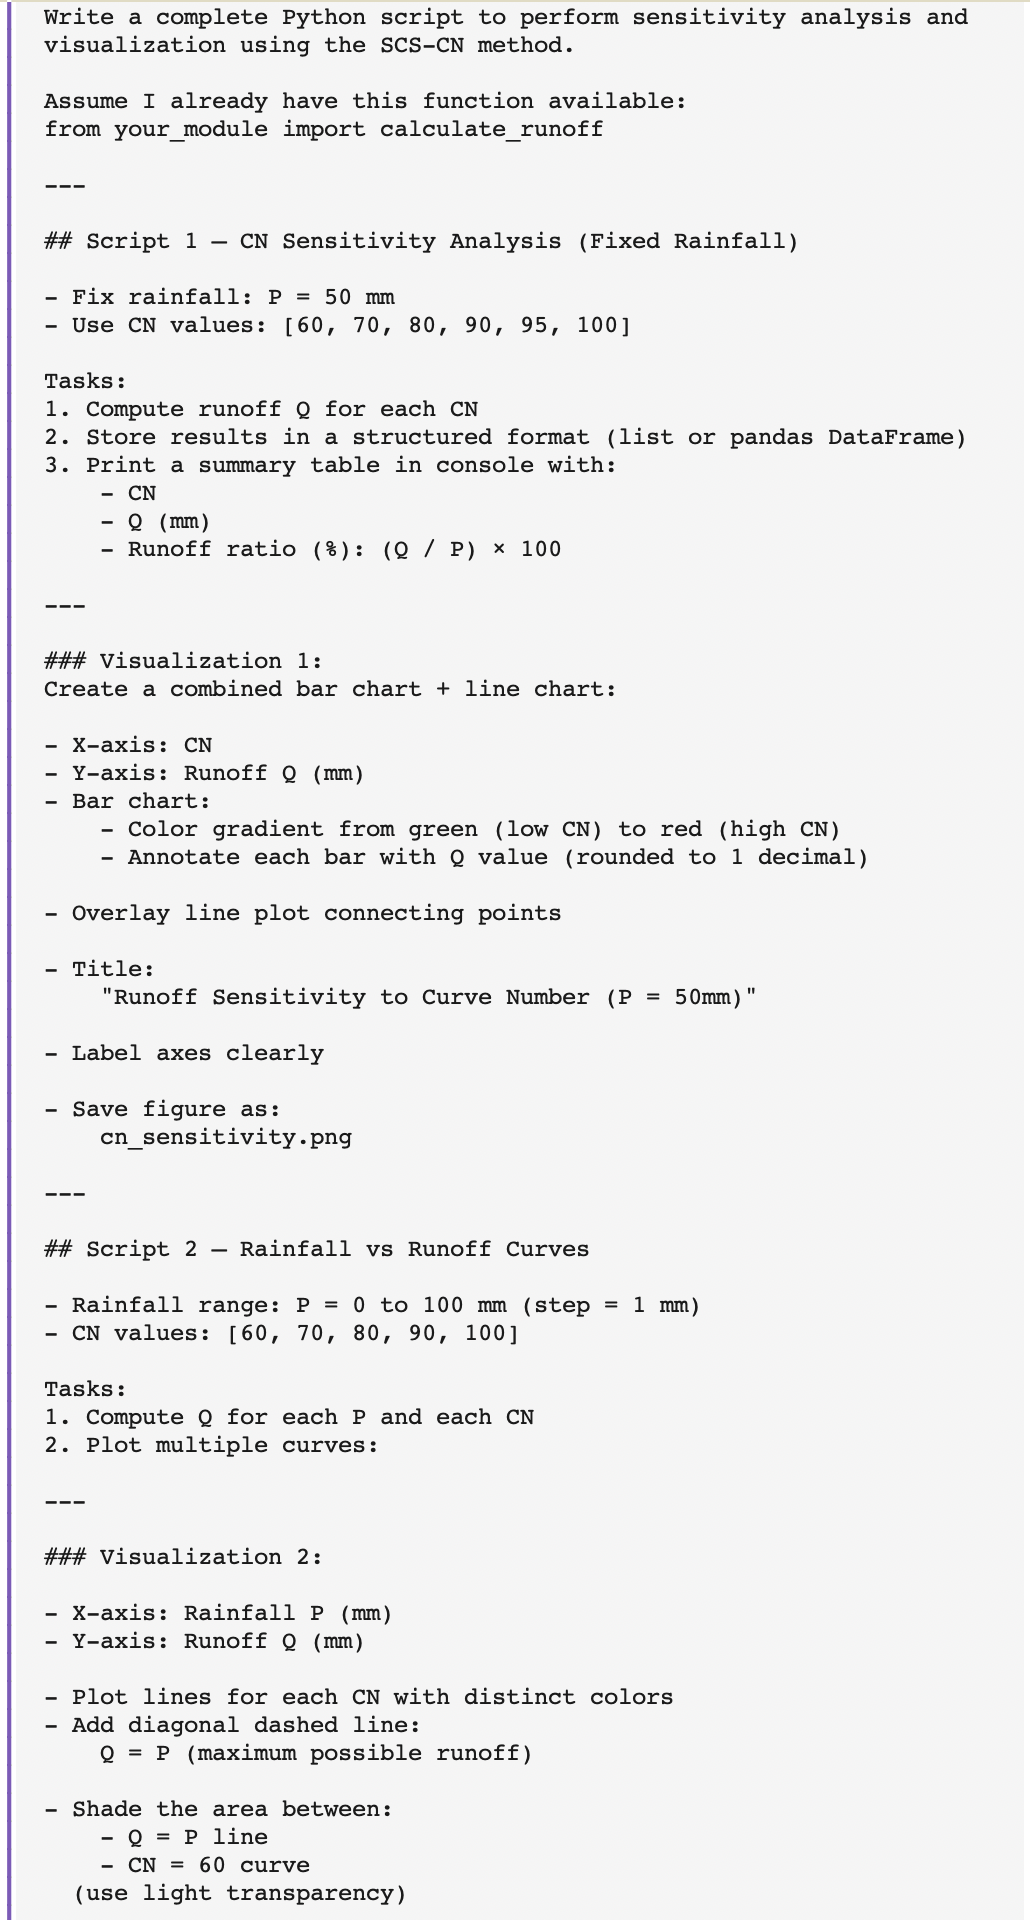
\includegraphics[width=0.9\textwidth]{experiment-2-prompt3-1.png}
    \caption{Initial prompt for sensitivity analysis (page 1)}
    \label{fig:p3prompt1}
\end{figure}

\begin{figure}[H]
    \centering
    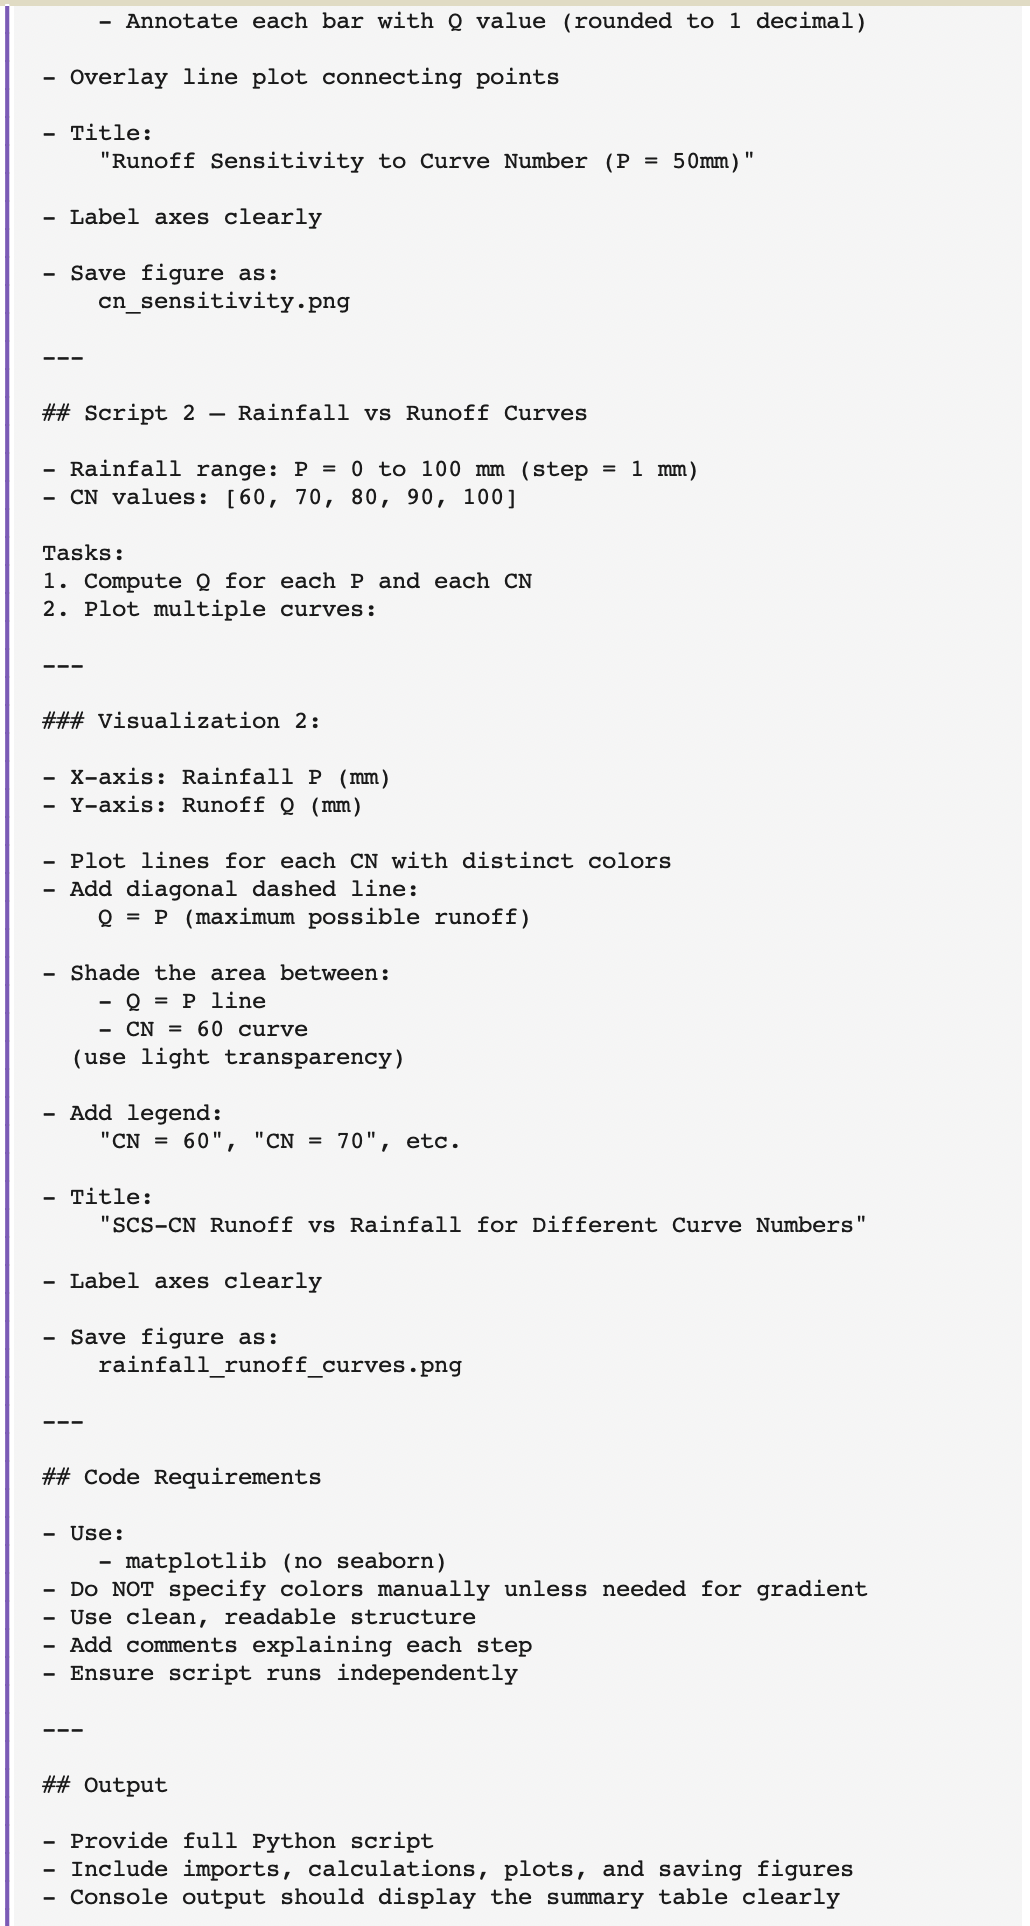
\includegraphics[width=0.9\textwidth]{experiment-2-prompt3-2.png}
    \caption{Initial prompt for sensitivity analysis (page 2)}
    \label{fig:p3prompt2}
\end{figure}

\subsection{Prompt Feedback}

\begin{figure}[H]
    \centering
    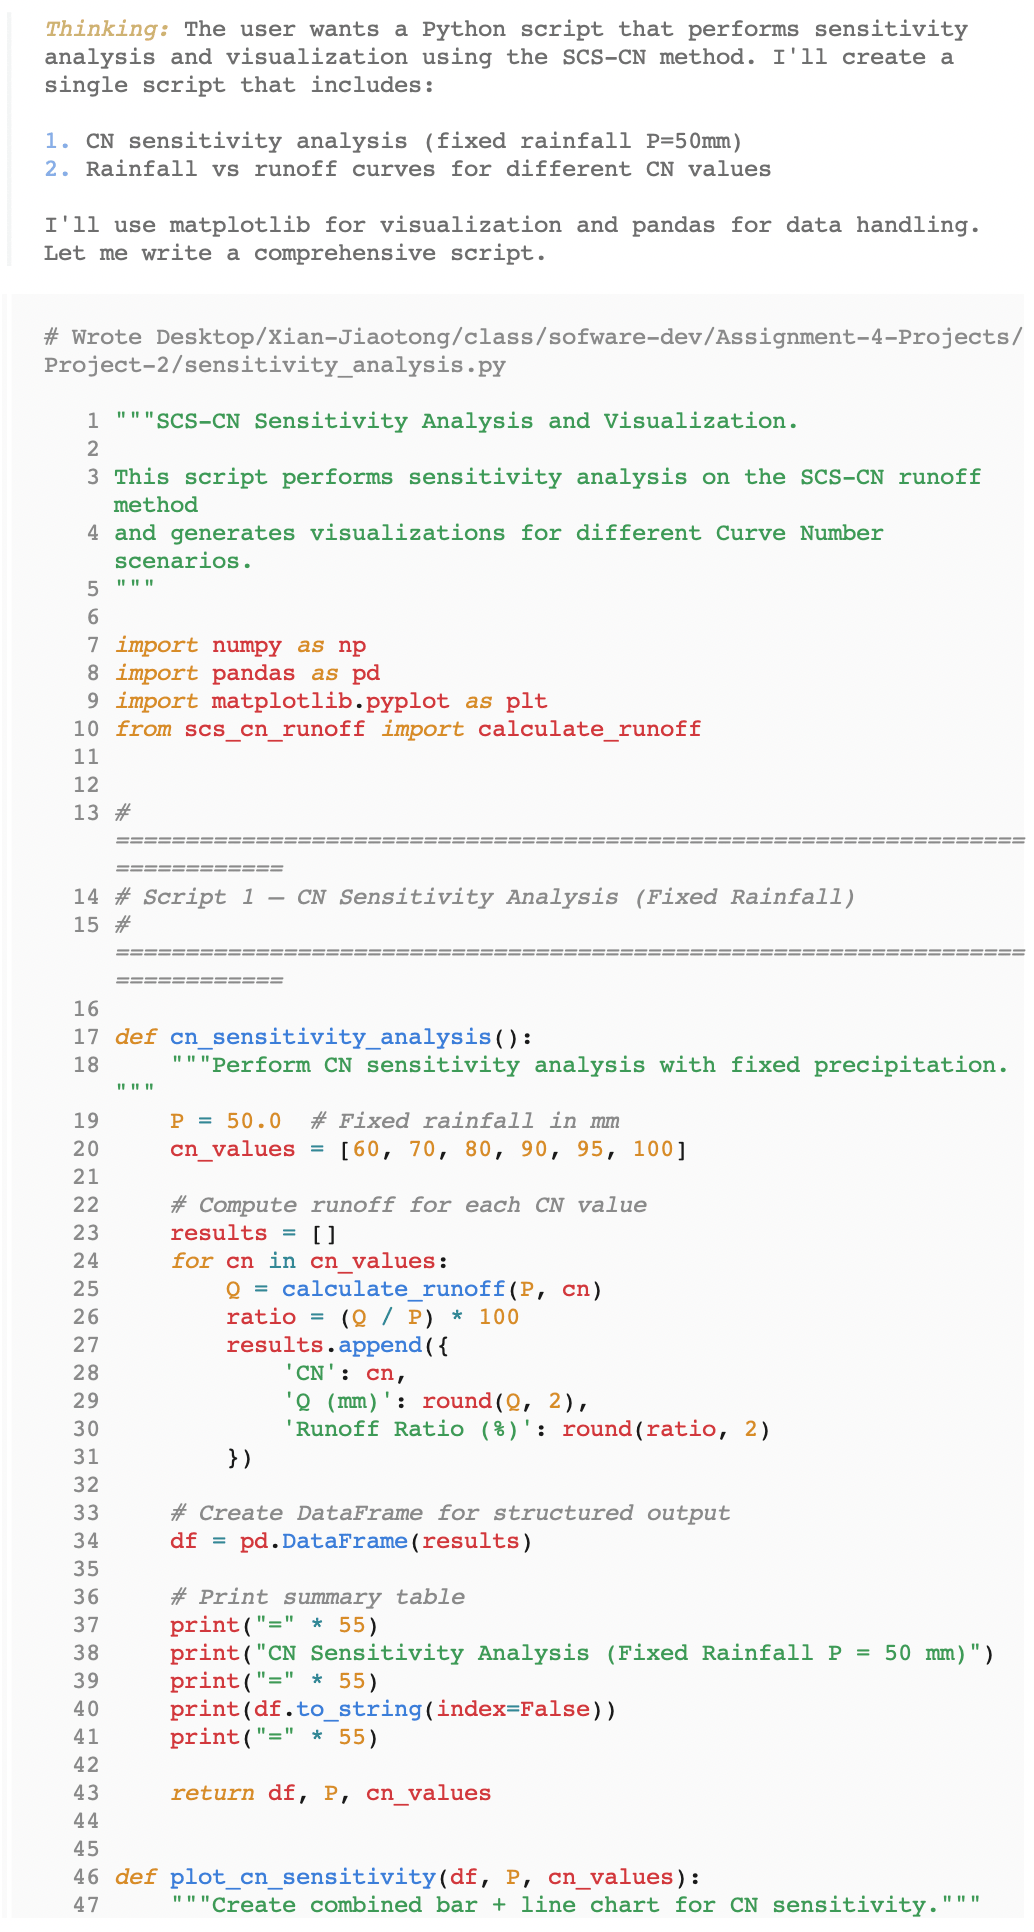
\includegraphics[width=0.9\textwidth]{experiment-2-prompt3-feedback1.png}
    \caption{Agent feedback for sensitivity analysis prompt (page 1)}
    \label{fig:p3fb1}
\end{figure}

\begin{figure}[H]
    \centering
    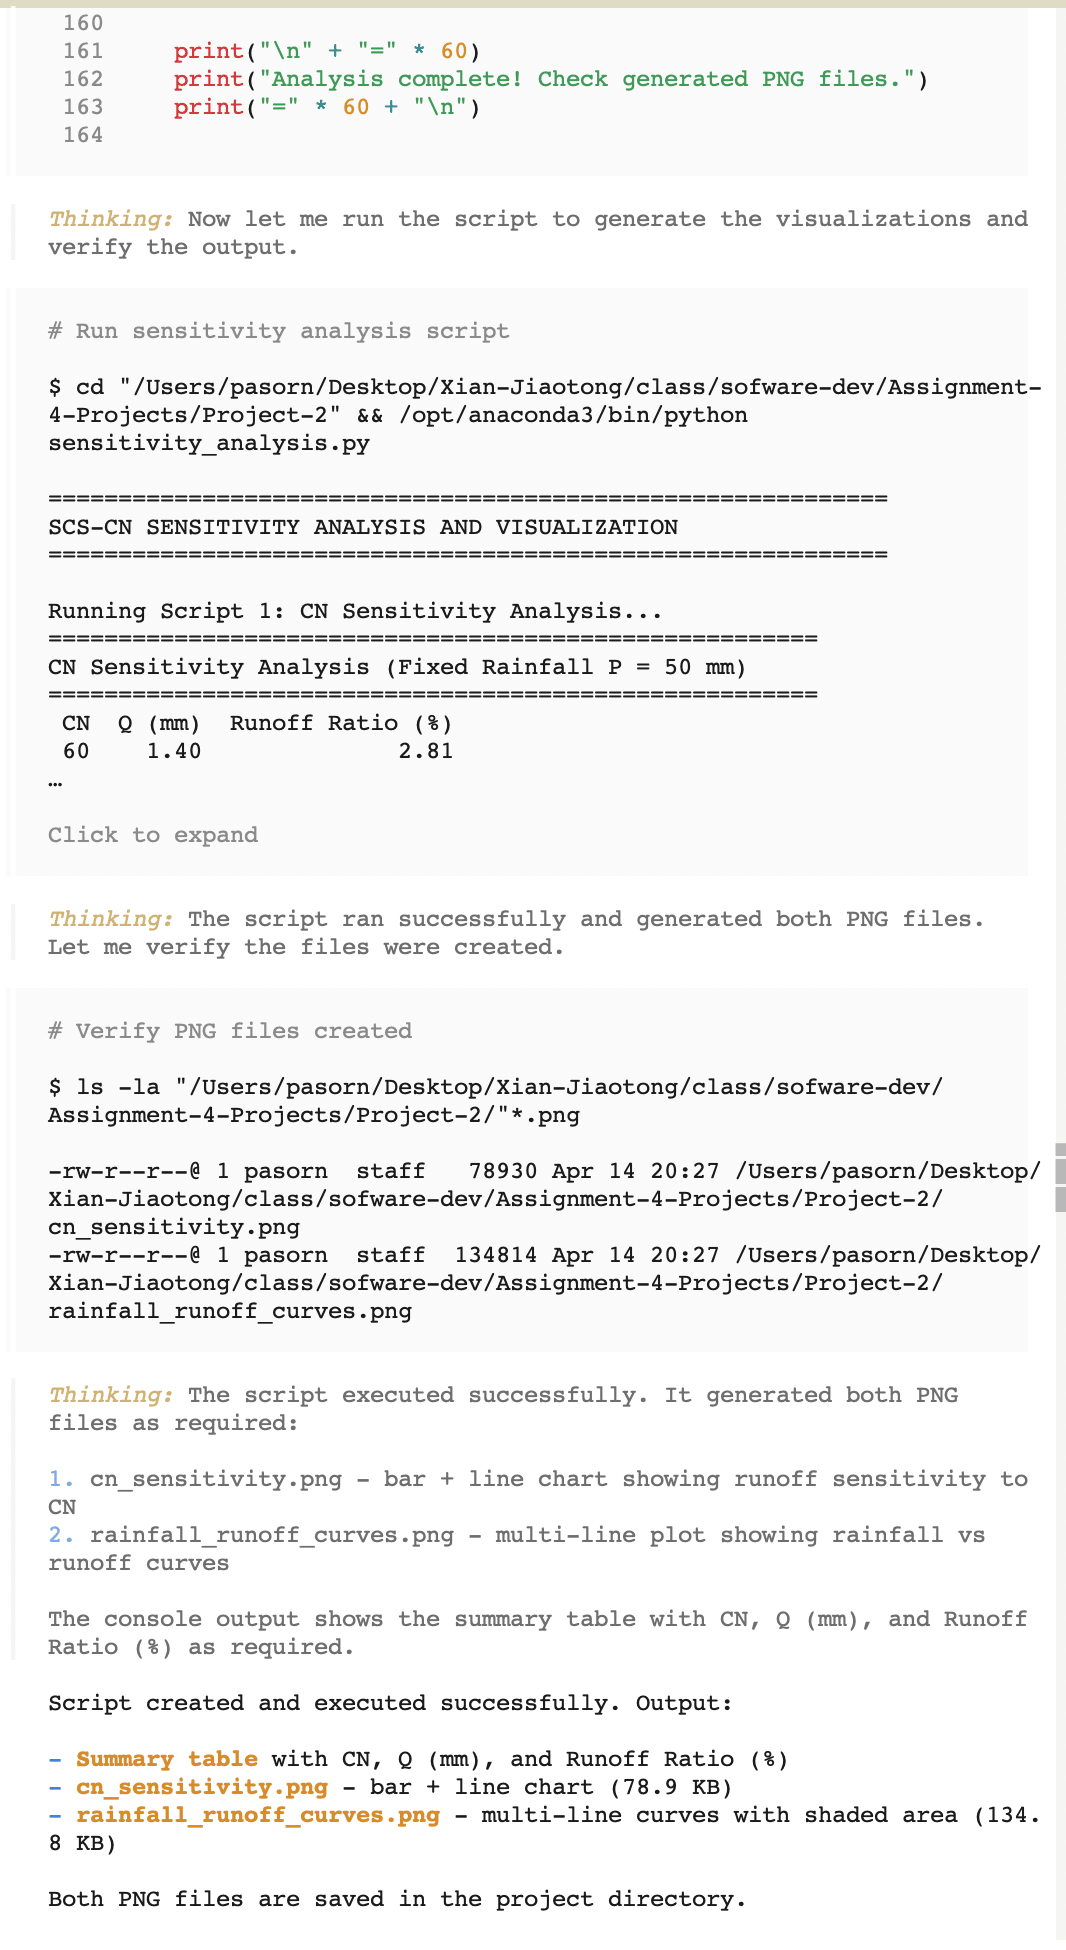
\includegraphics[width=0.9\textwidth]{experiment-2-prompt3-feedback2.png}
    \caption{Agent feedback for sensitivity analysis prompt (page 2)}
    \label{fig:p3fb2}
\end{figure}

\subsection{Result}

\begin{figure}[H]
    \centering
    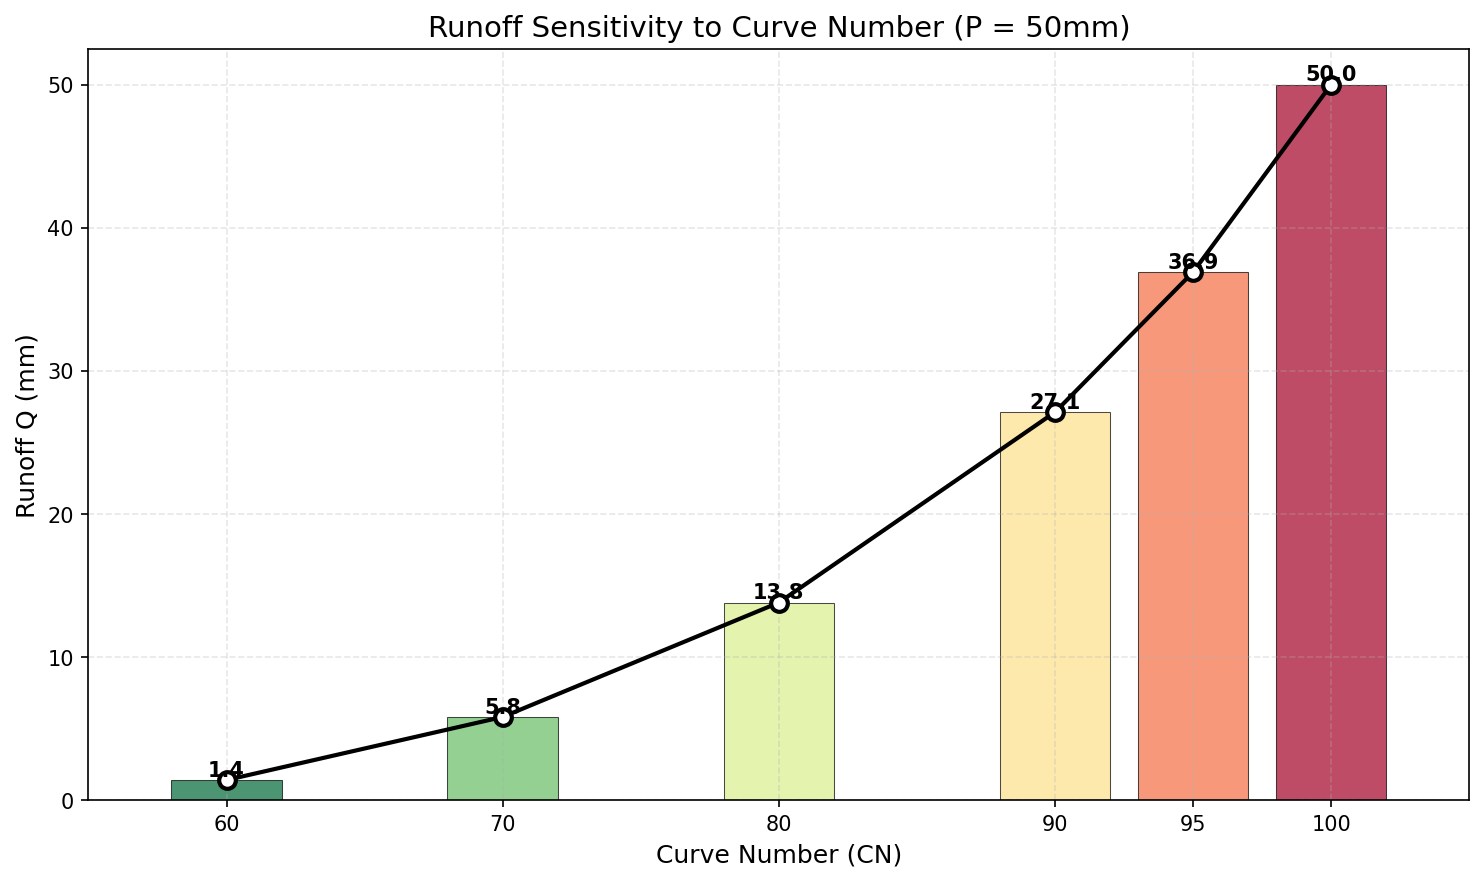
\includegraphics[width=0.9\textwidth]{cn_sensitivity.png}
    \caption{Sensitivity of runoff to Curve Number: $Q$ vs CN at fixed $P = 50$~mm}
    \label{fig:p3result1}
\end{figure}

\begin{figure}[H]
    \centering
    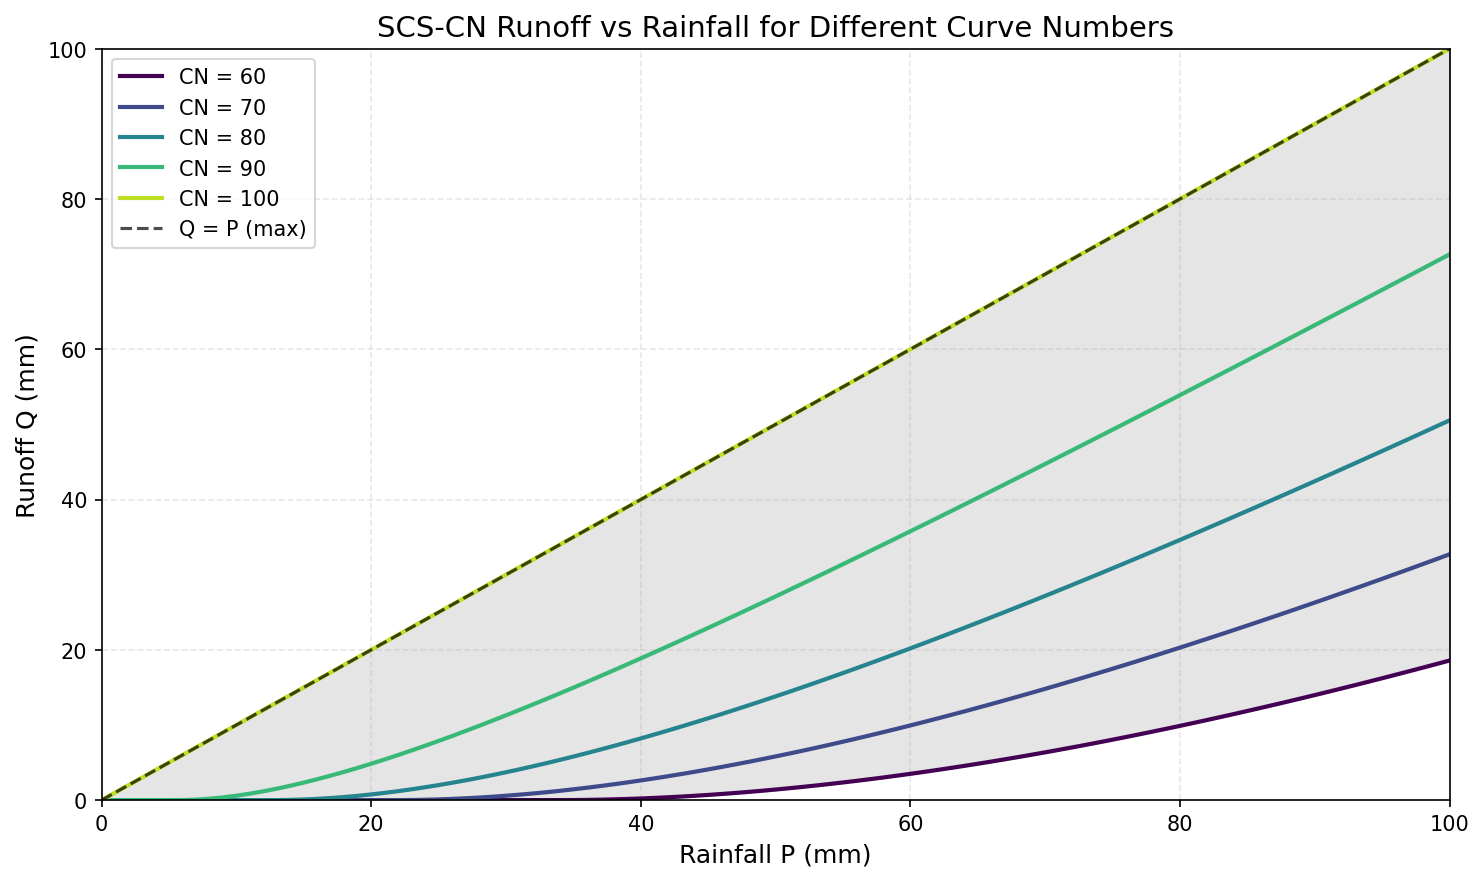
\includegraphics[width=0.9\textwidth]{rainfall_runoff_curves.png}
    \caption{Rainfall--runoff curves for selected CN values over $P \in [0, 200]$~mm}
    \label{fig:p3result2}
\end{figure}

Three observations follow from the sensitivity plots:
\begin{itemize}[leftmargin=1.8em]
    \item Runoff is a strictly increasing function of CN at fixed rainfall, consistent with the physical interpretation that higher CN reflects lower infiltration capacity.
    \item The CN--$Q$ relationship is markedly non-linear: incremental increases in CN above 90 produce disproportionately large increases in runoff, which explains the sensitivity of urbanizing watersheds to small changes in impervious cover.
    \item All curves asymptotically approach the line $Q = P$ as $P \to \infty$, with the impervious case ($\mathrm{CN} = 100$) reaching it immediately. This confirms the constraint $Q \leq P$ holds across the full parameter space.
\end{itemize}

%% ============================================================
\section{Validation \& Documentation}
\label{sec:validation}
%% ============================================================

This section verifies that the AI-generated implementation satisfies both mathematical correctness and physical realism. Validation is performed against the four constraints introduced in Section~2:
\begin{itemize}[leftmargin=1.8em]
    \item Runoff never exceeds rainfall ($Q \leq P$).
    \item No runoff occurs when $P < I_a$.
    \item Increasing CN at fixed $P$ produces non-decreasing $Q$ (monotonicity).
    \item The numerical result for the worked example ($P = 50$, $\mathrm{CN} = 80$) matches the expected value of 13.8~mm.
\end{itemize}

All AI interactions throughout the experiment are documented in \texttt{prompt\_log.md} to support reproducibility and to enable post-hoc analysis of the prompt-engineering process.

\subsection{Initial Prompt}

\begin{figure}[H]
    \centering
    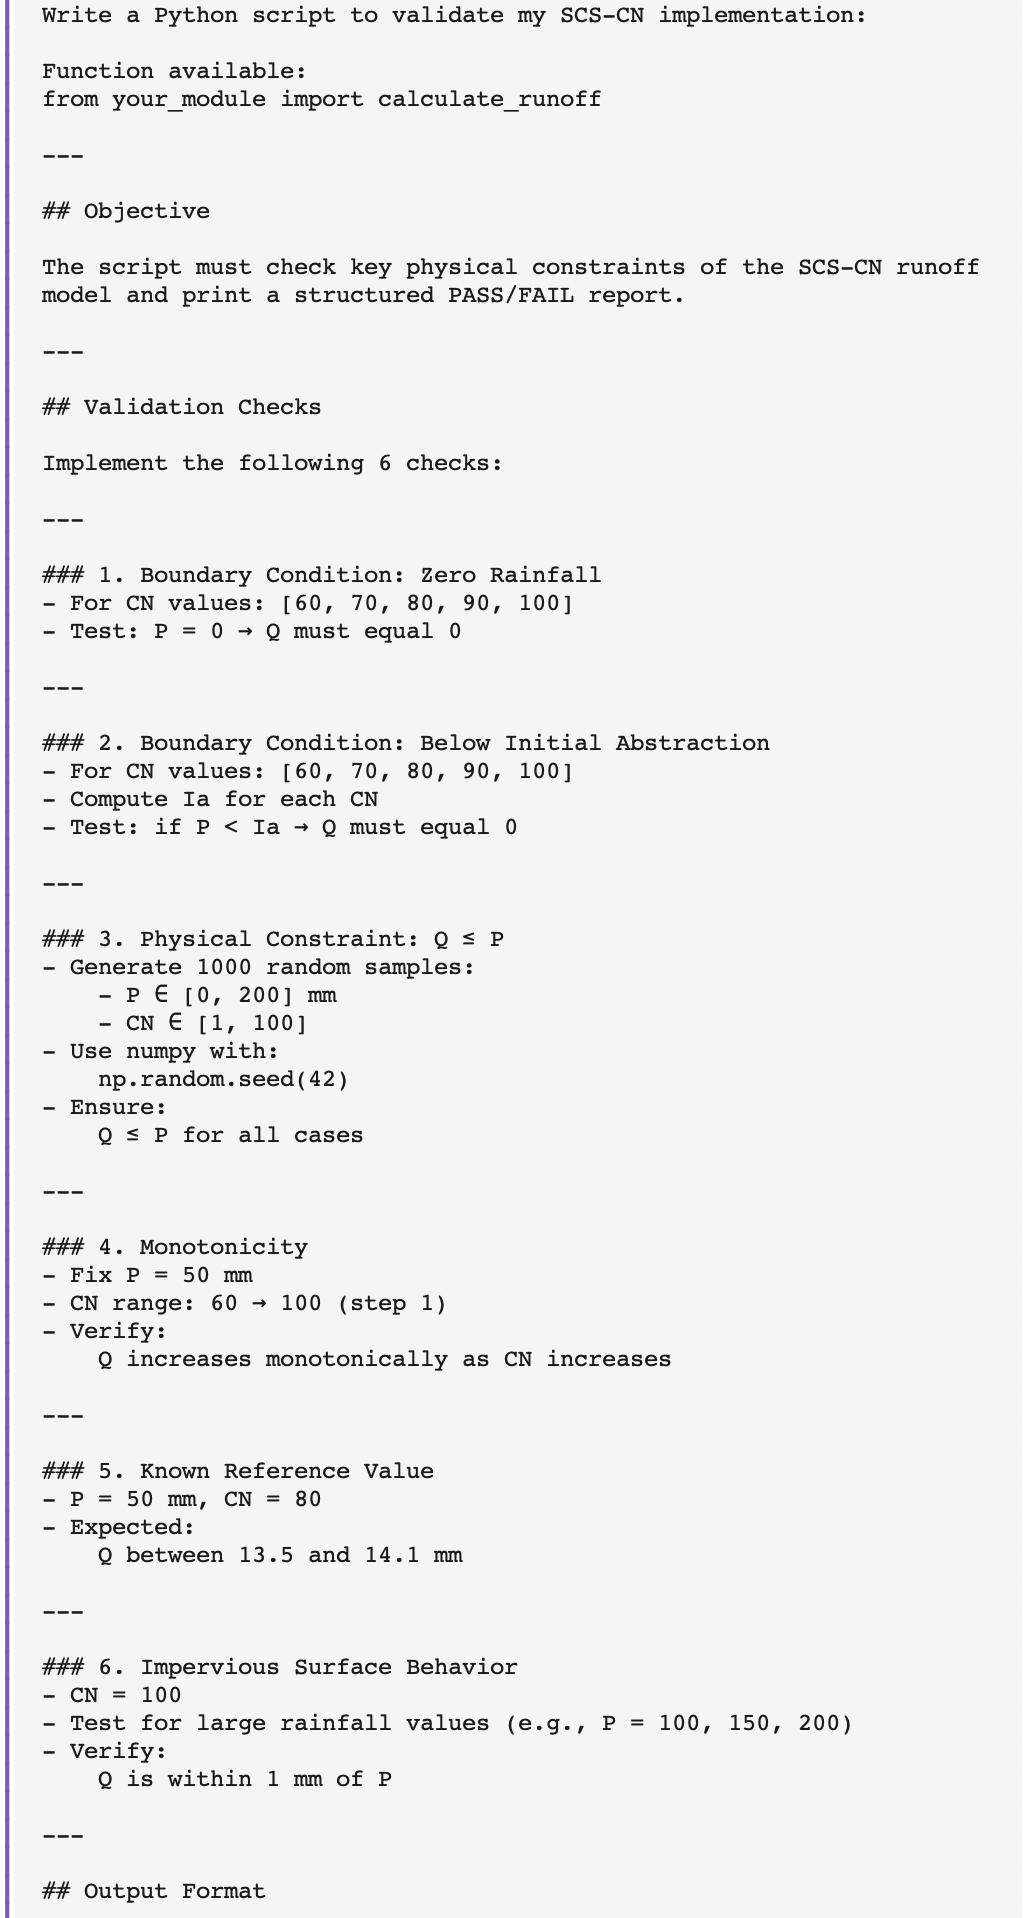
\includegraphics[width=0.9\textwidth]{experiment-2-prompt4-1.png}
    \caption{Initial validation prompt (page 1)}
    \label{fig:p4prompt1}
\end{figure}

\begin{figure}[H]
    \centering
    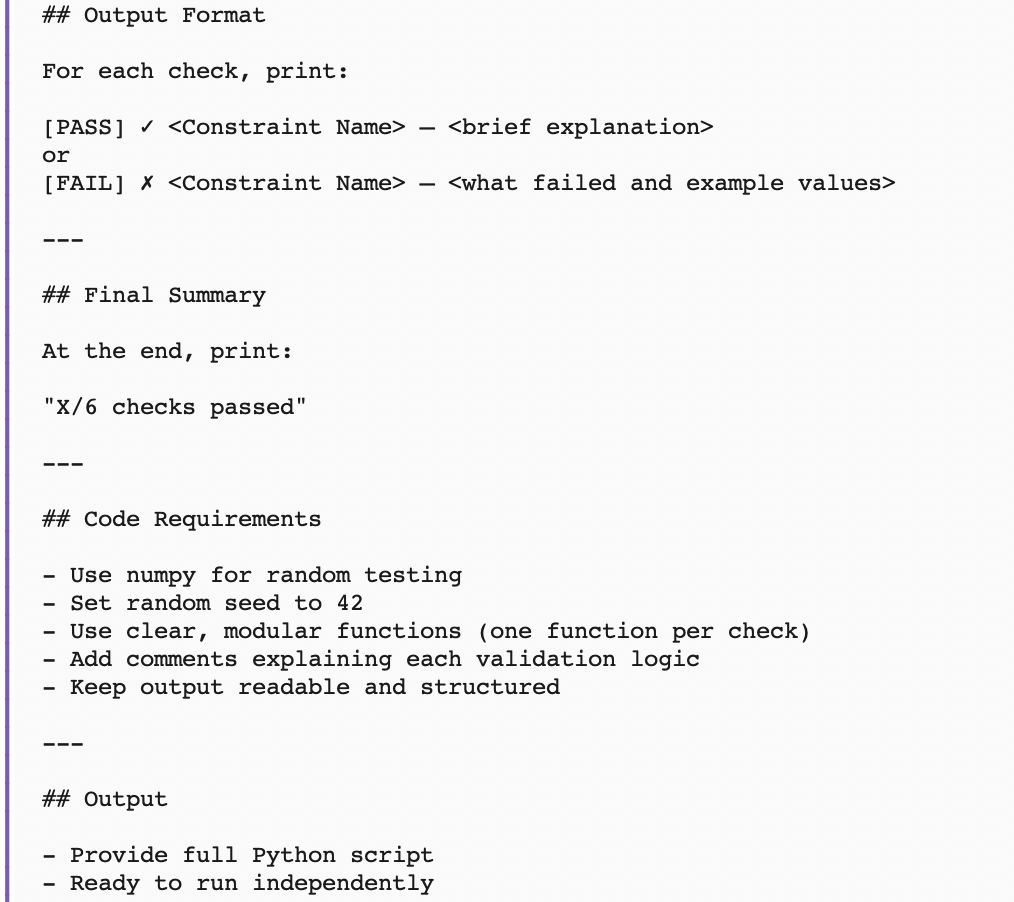
\includegraphics[width=0.9\textwidth]{experiment-2-prompt4-2.png}
    \caption{Initial validation prompt (page 2)}
    \label{fig:p4prompt2}
\end{figure}

\subsection{Prompt Feedback}

\begin{figure}[H]
    \centering
    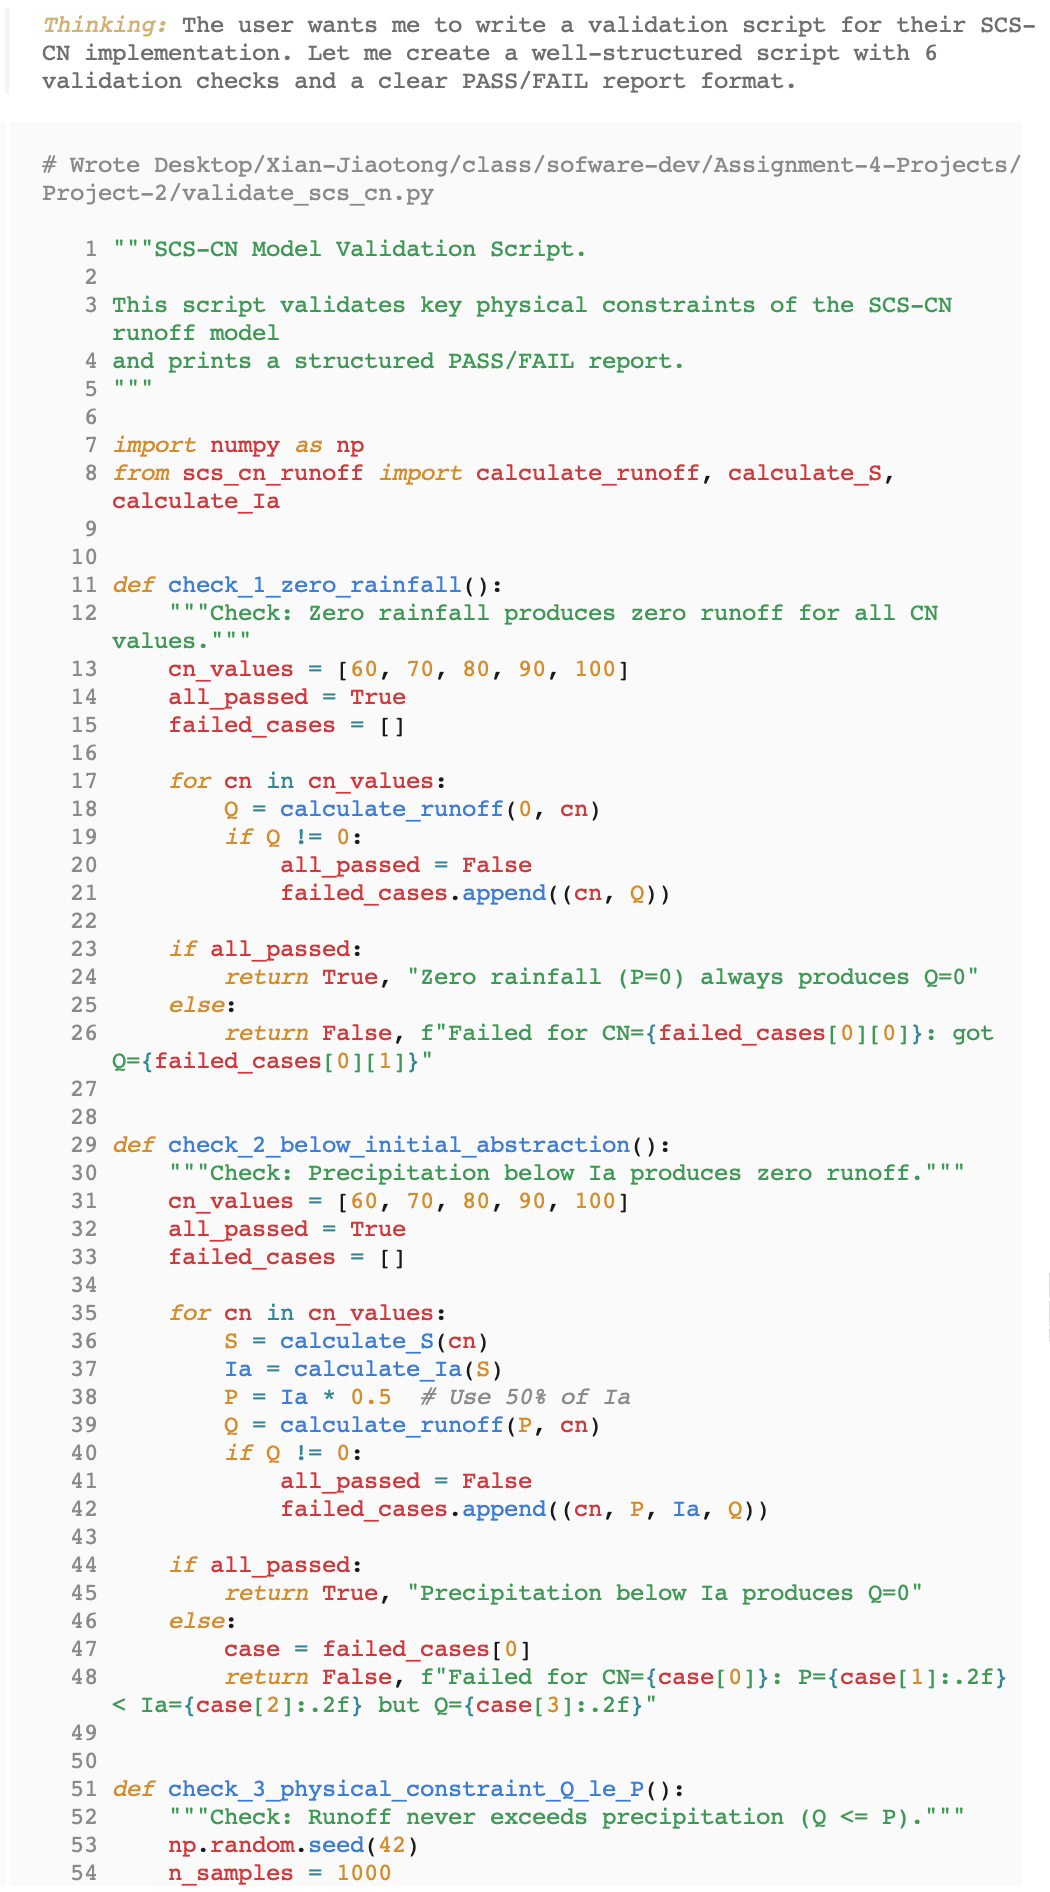
\includegraphics[width=0.9\textwidth]{experiment-2-prompt4-feedback1.png}
    \caption{Correction of logical and physical inconsistencies (page 1)}
    \label{fig:p4fb1}
\end{figure}

\begin{figure}[H]
    \centering
    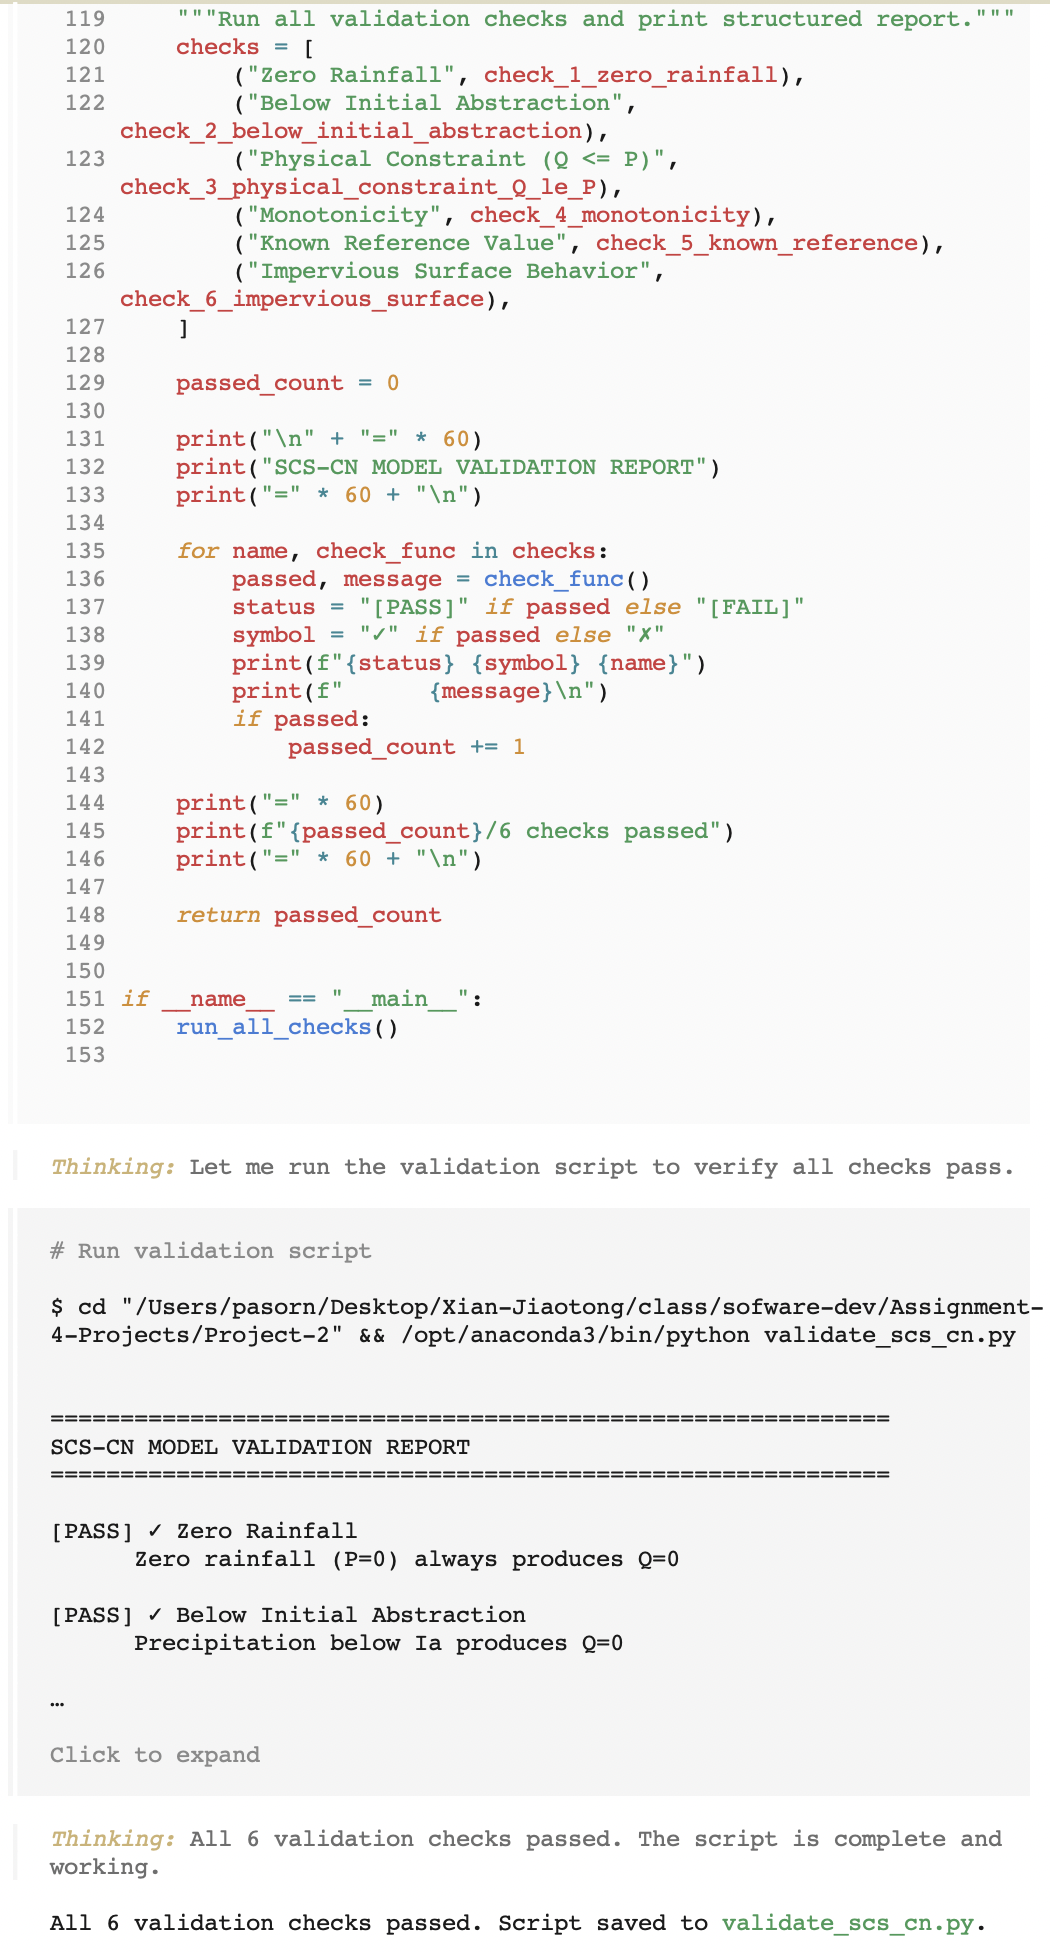
\includegraphics[width=0.9\textwidth]{experiment-2-prompt4-feedback2.png}
    \caption{Correction of logical and physical inconsistencies (page 2)}
    \label{fig:p4fb2}
\end{figure}

\subsection{Result}

\begin{figure}[H]
    \centering
    \includegraphics[width=0.9\textwidth]{result-prompt4.png}
    \caption{Final validated implementation, all physical constraints verified}
    \label{fig:p4result}
\end{figure}

The validation process underscores the importance of domain knowledge when working with AI-generated code: the agent occasionally produced syntactically correct but physically implausible outputs (e.g., omitting the $Q \leq P$ guard), which were detected only by explicit reference to the governing equations.

%% ============================================================
\section{Extensions}
%% ============================================================

This section explores advanced improvements beyond the base implementation, demonstrating the scalability of the AI-assisted development workflow. The proposed extensions are:
\begin{itemize}[leftmargin=1.8em]
    \item \textbf{Time--area method} for distributed watershed routing, allowing spatial heterogeneity of CN within a basin.
    \item \textbf{Antecedent Moisture Condition (AMC) adjustments} that modify CN based on prior 5-day rainfall, switching between AMC-I (dry), AMC-II (average), and AMC-III (wet) regimes.
    \item \textbf{Interactive visualization} with parameter sliders for $P$ and CN, implemented using \texttt{ipywidgets}.
    \item \textbf{Comparative analysis} between SCS-CN and the Rational method for small urban catchments.
\end{itemize}

\subsection{Initial Prompt}

\begin{figure}[H]
    \centering
    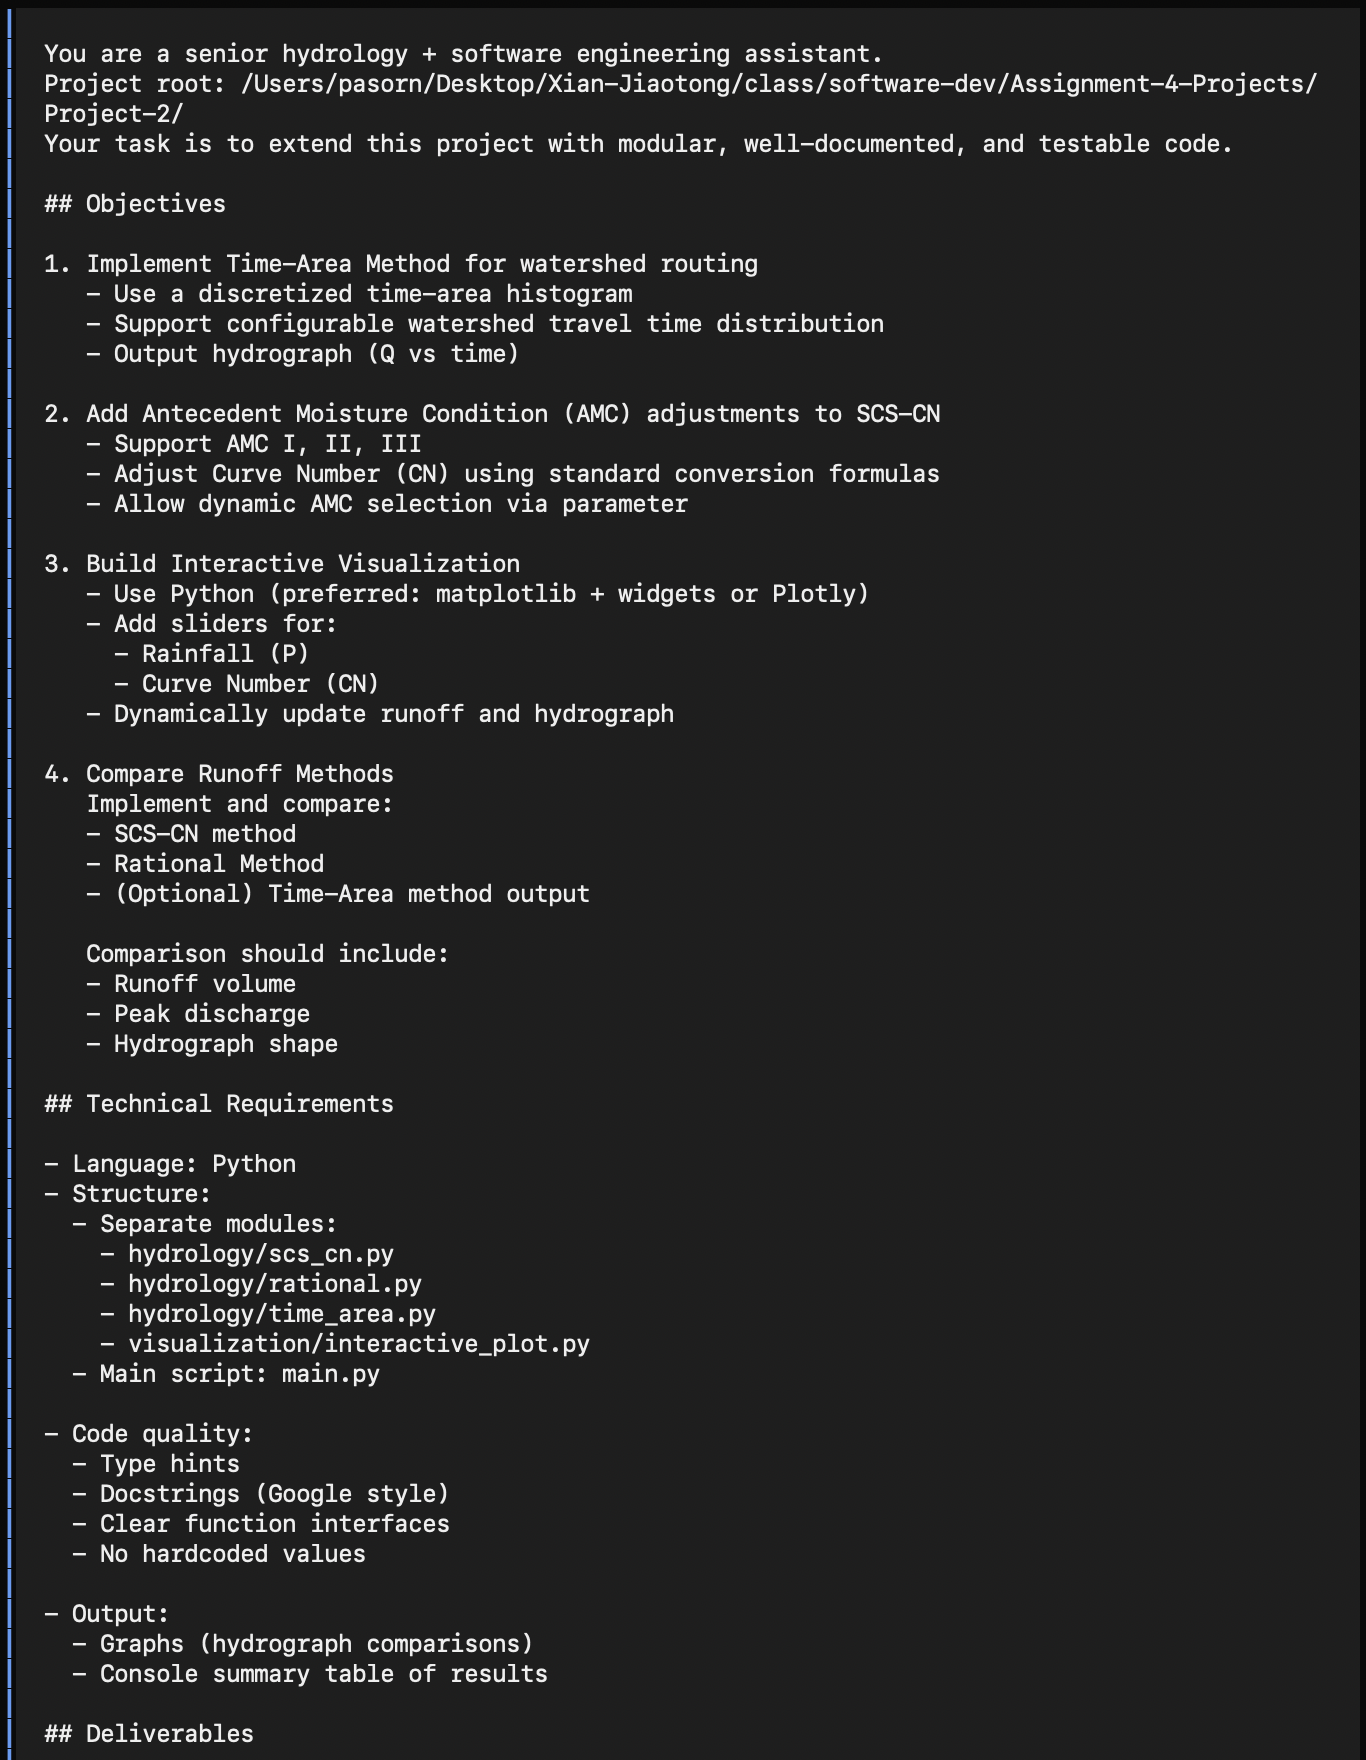
\includegraphics[width=0.9\textwidth]{experiment-2-prompt6-1.png}
    \caption{Prompt for extended features (page 1)}
    \label{fig:p6prompt1}
\end{figure}

\begin{figure}[H]
    \centering
    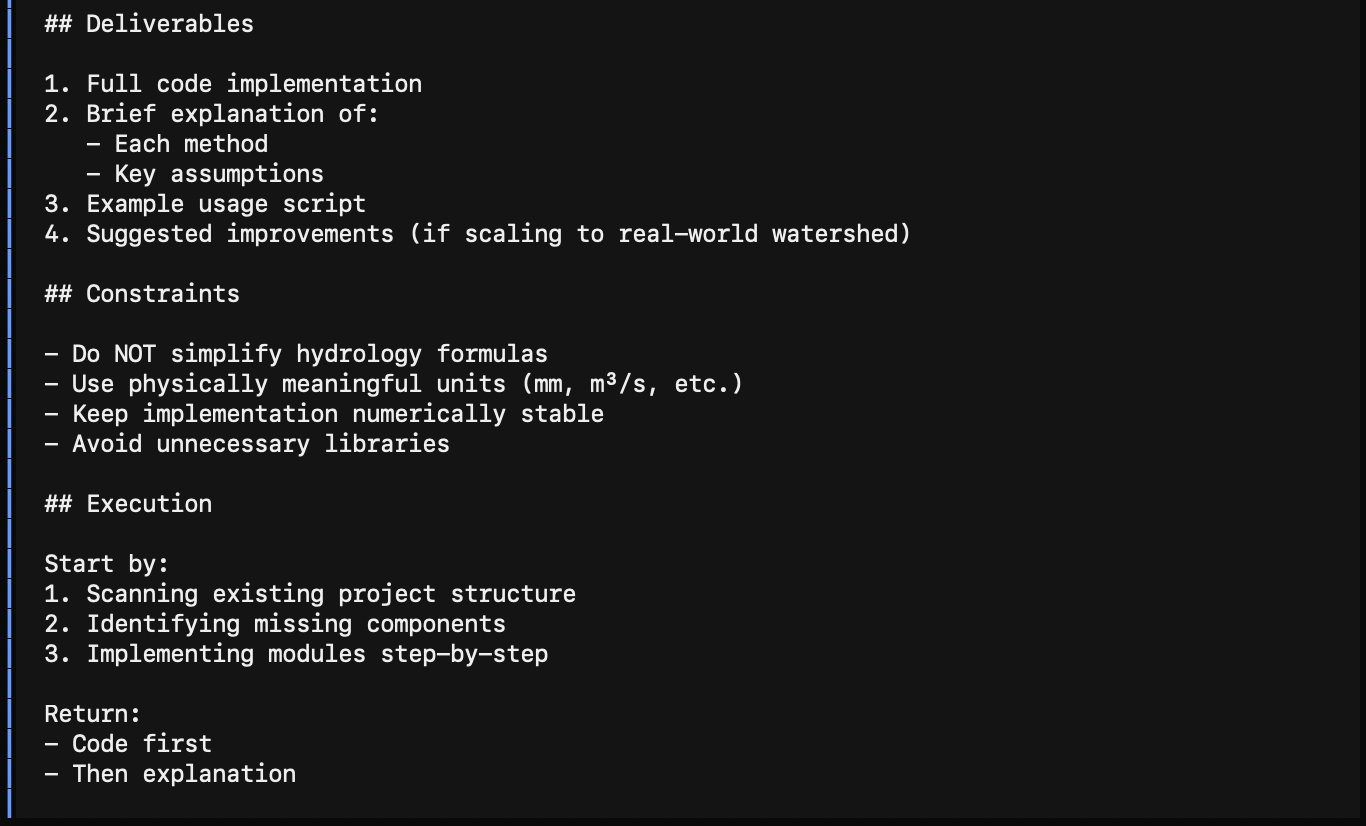
\includegraphics[width=0.9\textwidth]{experiment-2-prompt6-2.png}
    \caption{Prompt for extended features (page 2)}
    \label{fig:p6prompt2}
\end{figure}

\subsection{Prompt Feedback}

\begin{figure}[H]
    \centering
    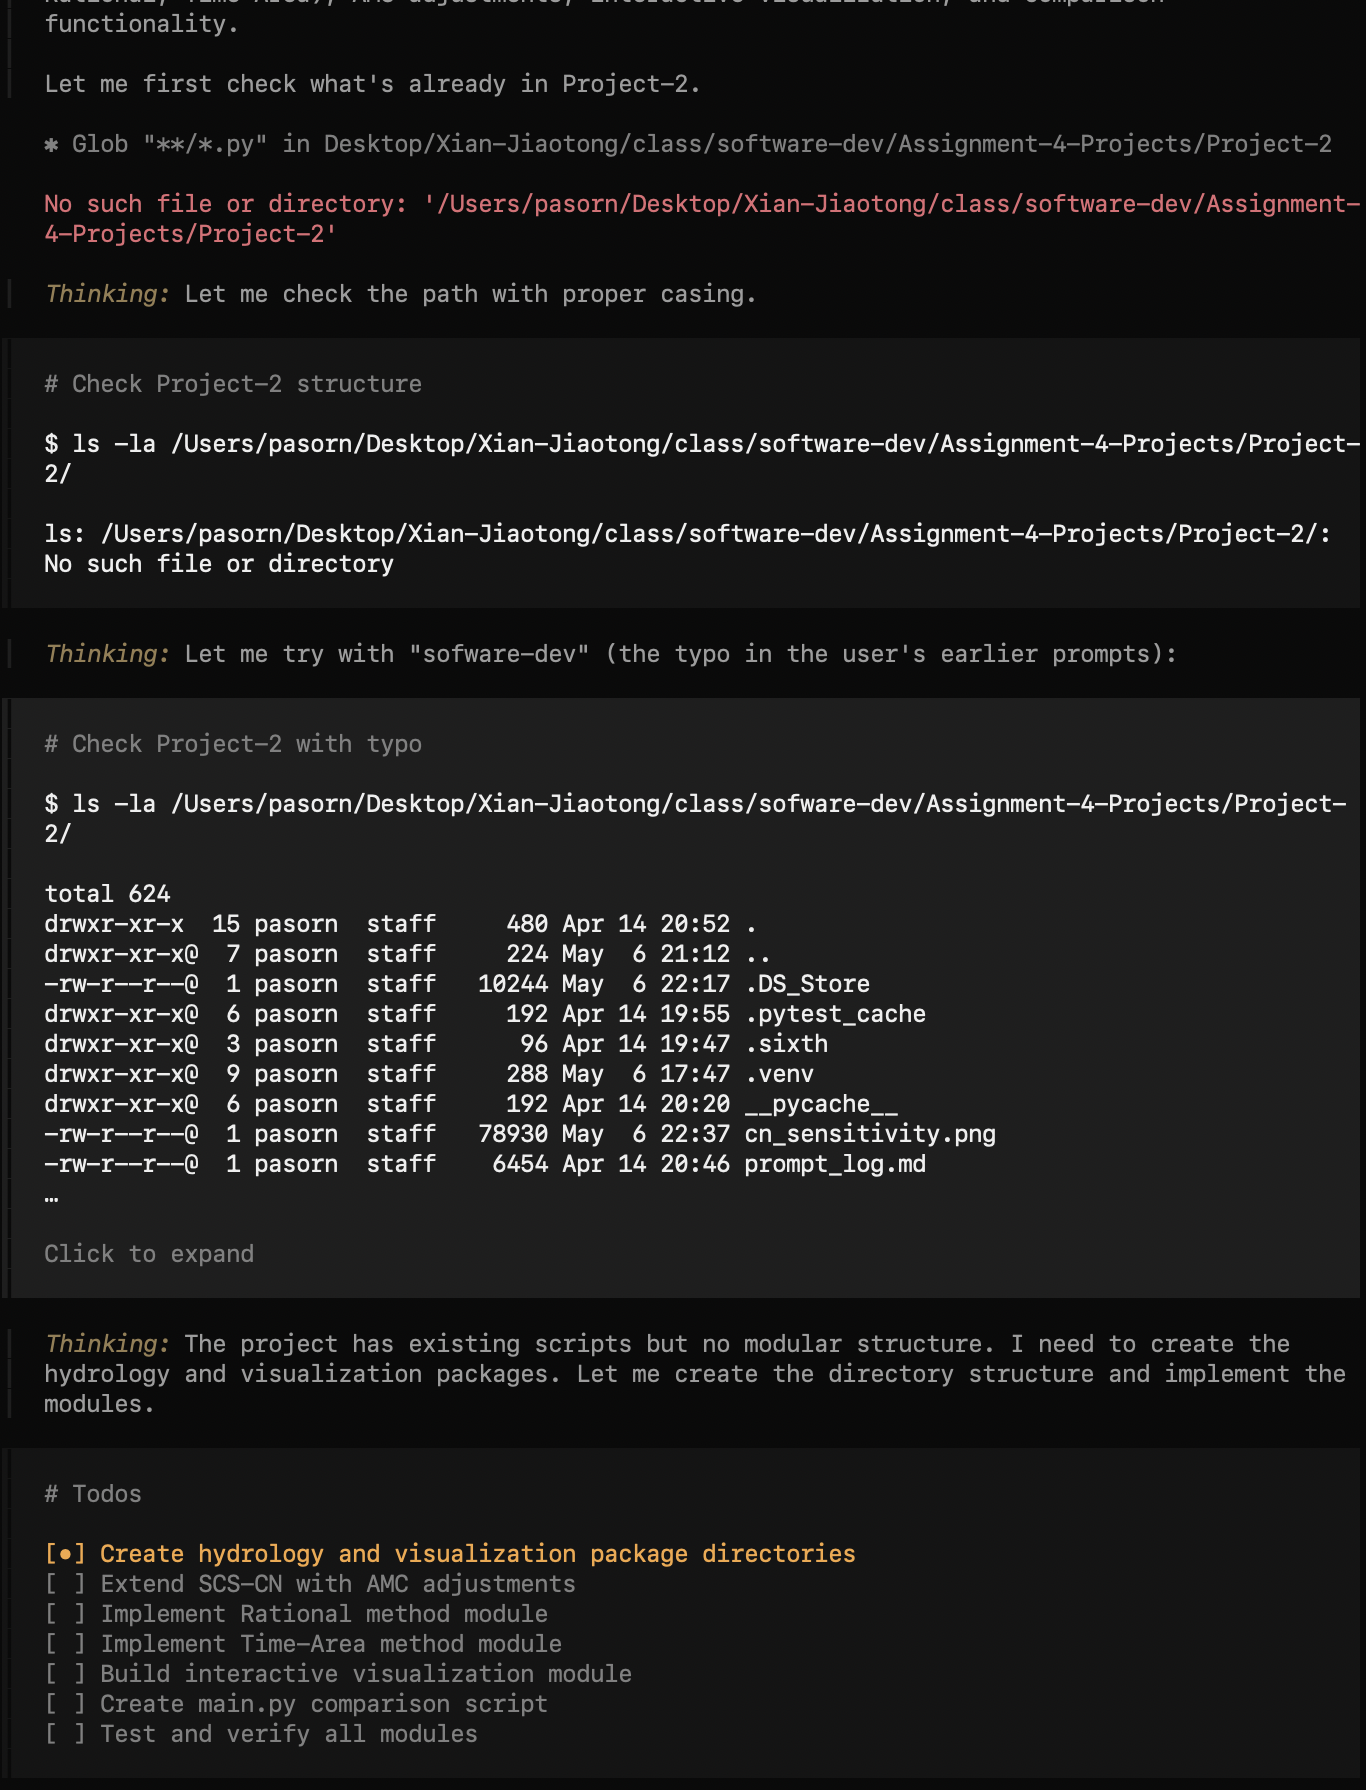
\includegraphics[width=0.9\textwidth]{experiment-2-prompt6-feedback1.png}
    \caption{Refinement of extension design (page 1)}
    \label{fig:p6fb1}
\end{figure}

\begin{figure}[H]
    \centering
    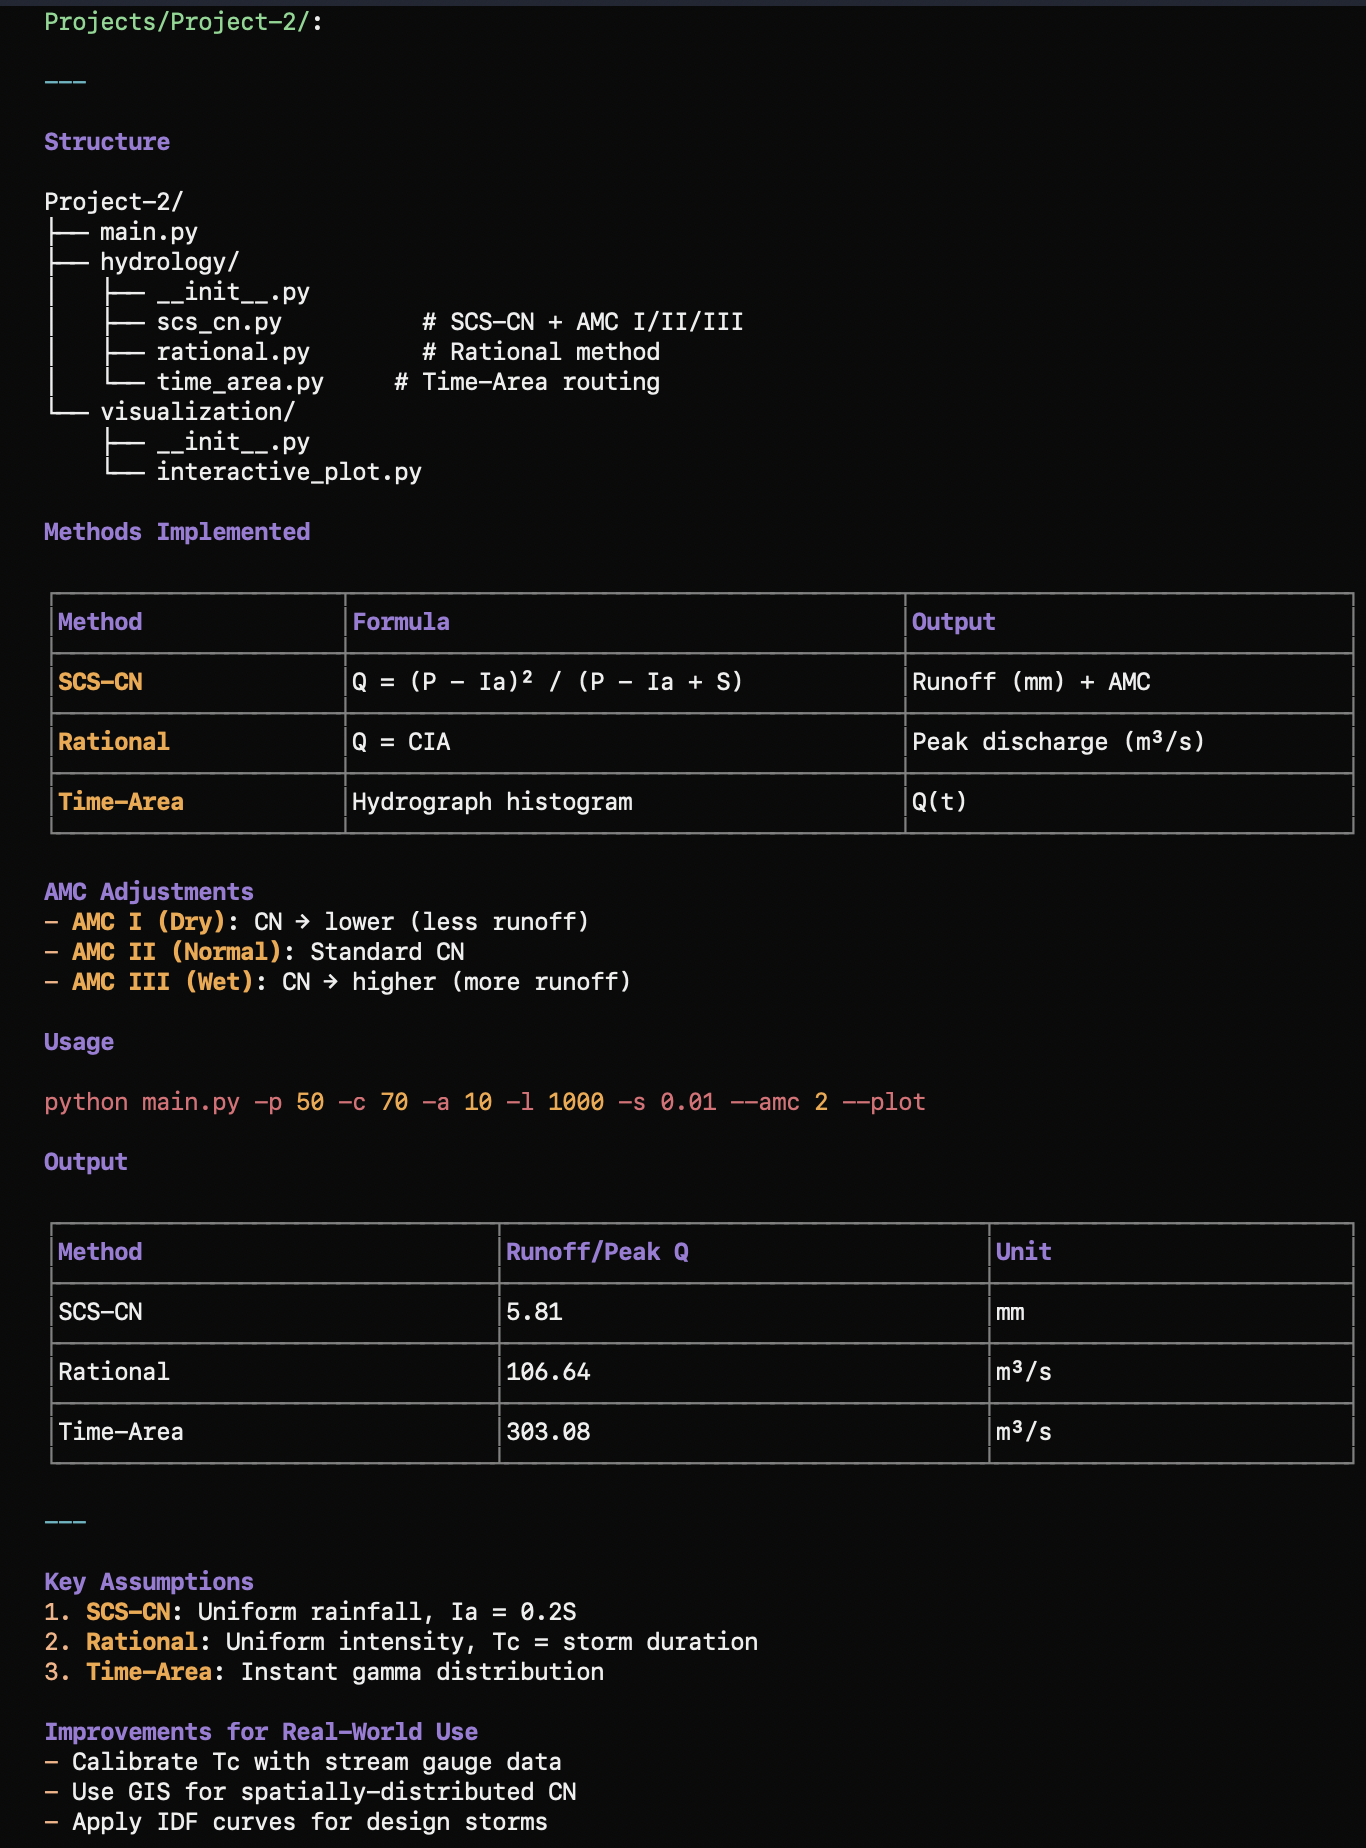
\includegraphics[width=0.9\textwidth]{experiment-2-prompt6-feedback14.png}
    \caption{Refinement of extension design (final iteration)}
    \label{fig:p6fb14}
\end{figure}

\subsection{Result}

\begin{figure}[H]
    \centering
    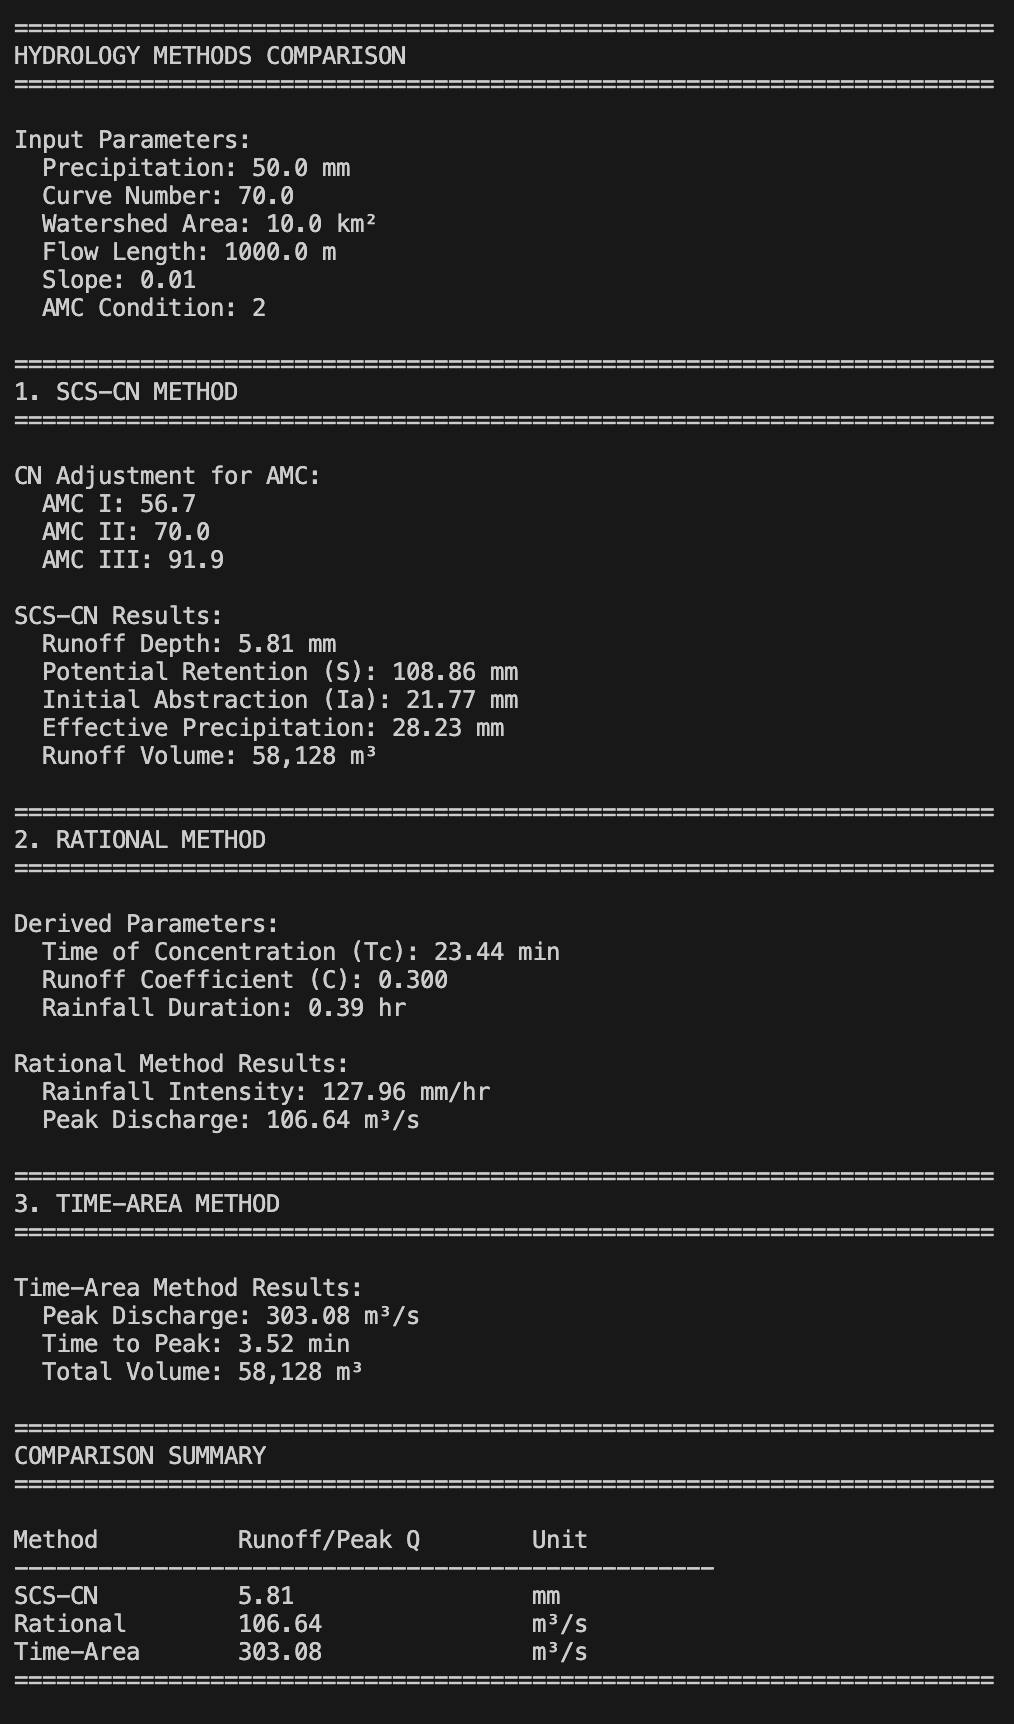
\includegraphics[width=0.9\textwidth]{experiment-2-prompt6-output.png}
    \caption{Extended implementation features}
    \label{fig:p6result}
\end{figure}

These extensions illustrate that the same prompt-driven workflow used for the base model generalizes naturally to richer hydrological formulations.

%% ============================================================
\section{Prompt Logging}
%% ============================================================

To ensure full reproducibility of the AI-assisted workflow, every user prompt and agent response was archived to \texttt{prompt\_log.md} in chronological order. This log serves both as an audit trail and as a teaching artifact that captures the evolution of prompt engineering across the experiment.

\subsection{Initial Prompt}

\begin{figure}[H]
    \centering
    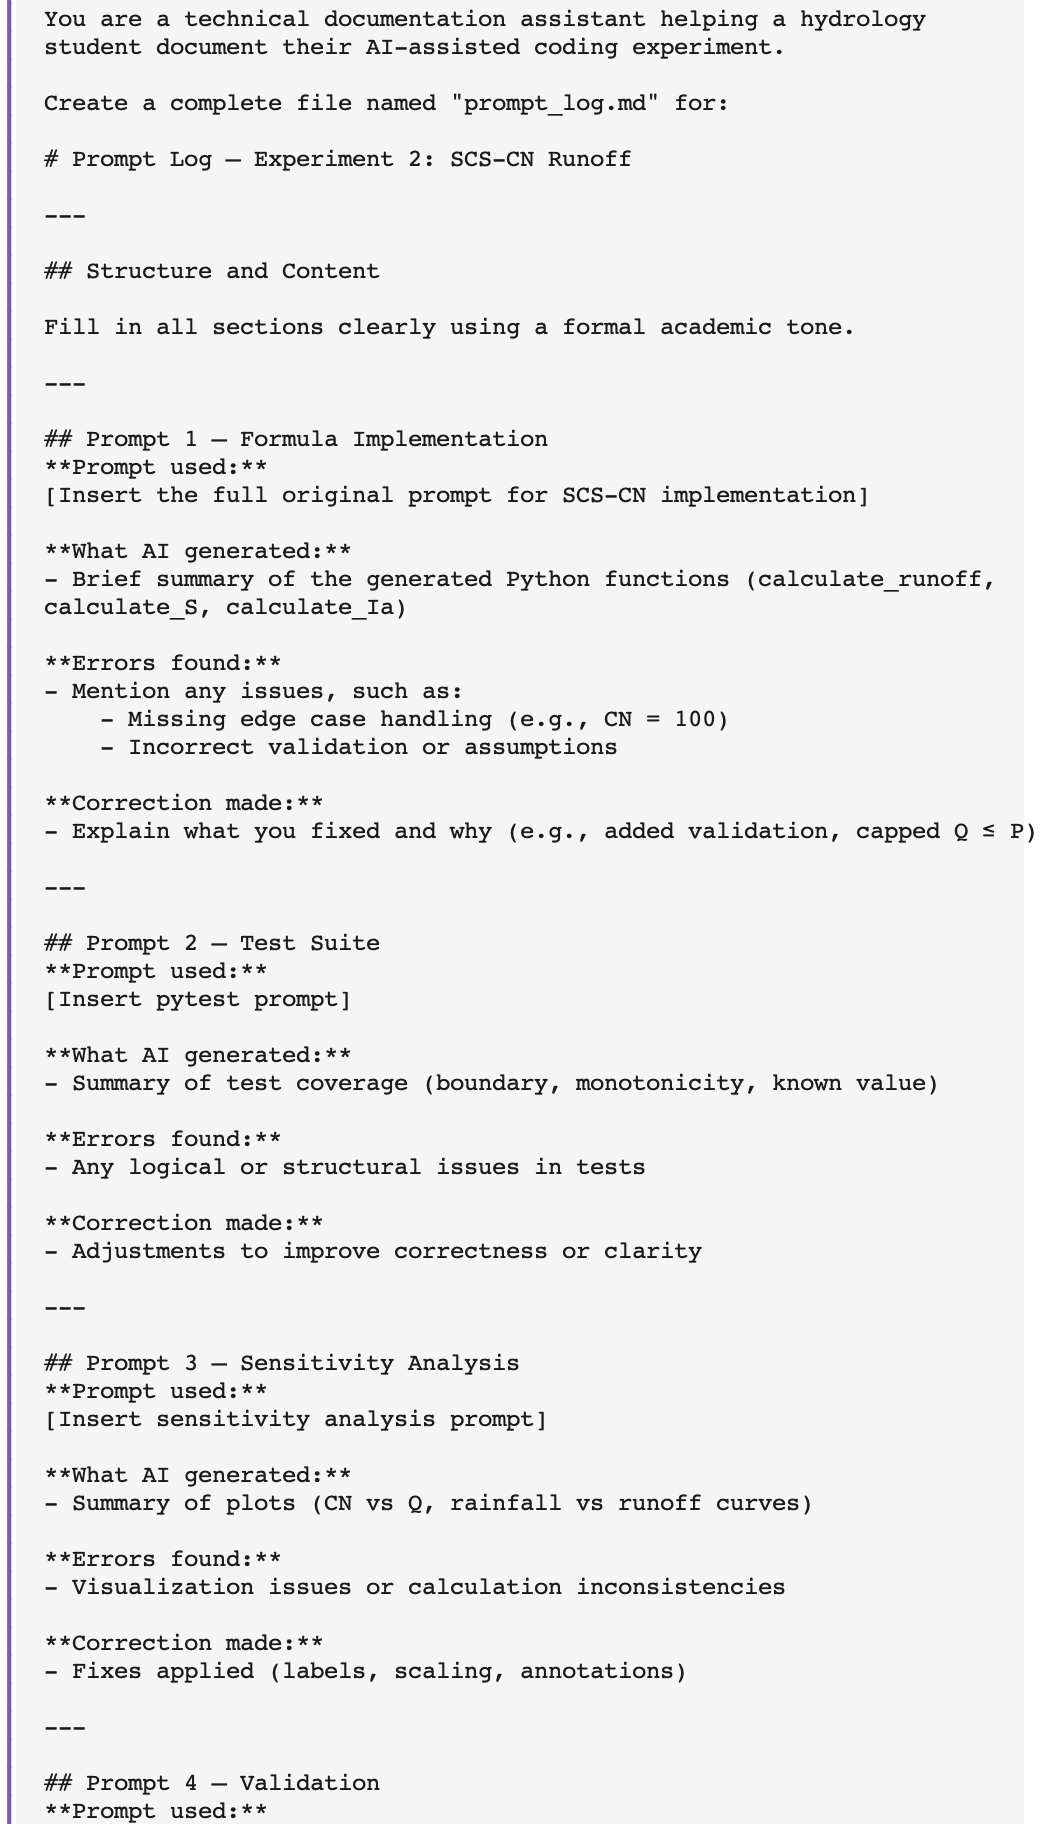
\includegraphics[width=0.9\textwidth]{experiment-2-prompt5-1.png}
    \caption{Initial prompt to archive all user prompts to \texttt{prompt\_log.md} (page 1)}
    \label{fig:p5prompt1}
\end{figure}

\begin{figure}[H]
    \centering
    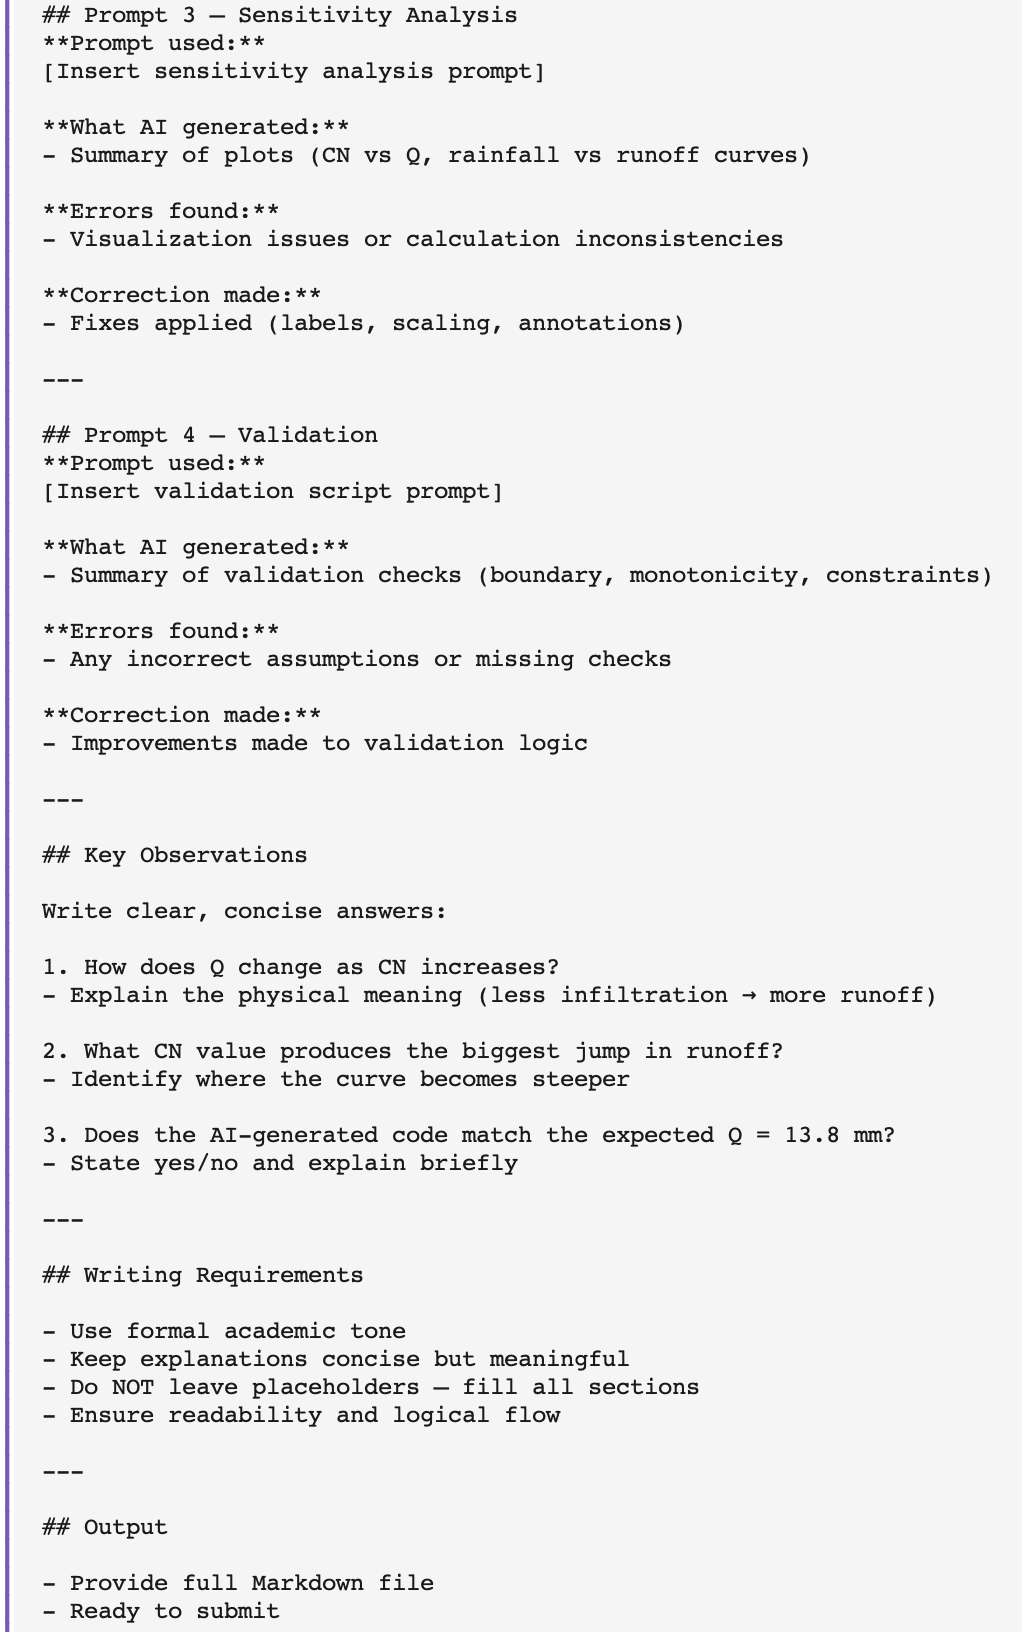
\includegraphics[width=0.9\textwidth]{experiment-2-prompt5-2.png}
    \caption{Initial prompt to archive all user prompts to \texttt{prompt\_log.md} (page 2)}
    \label{fig:p5prompt2}
\end{figure}

\subsection{Prompt Feedback}

\begin{figure}[H]
    \centering
    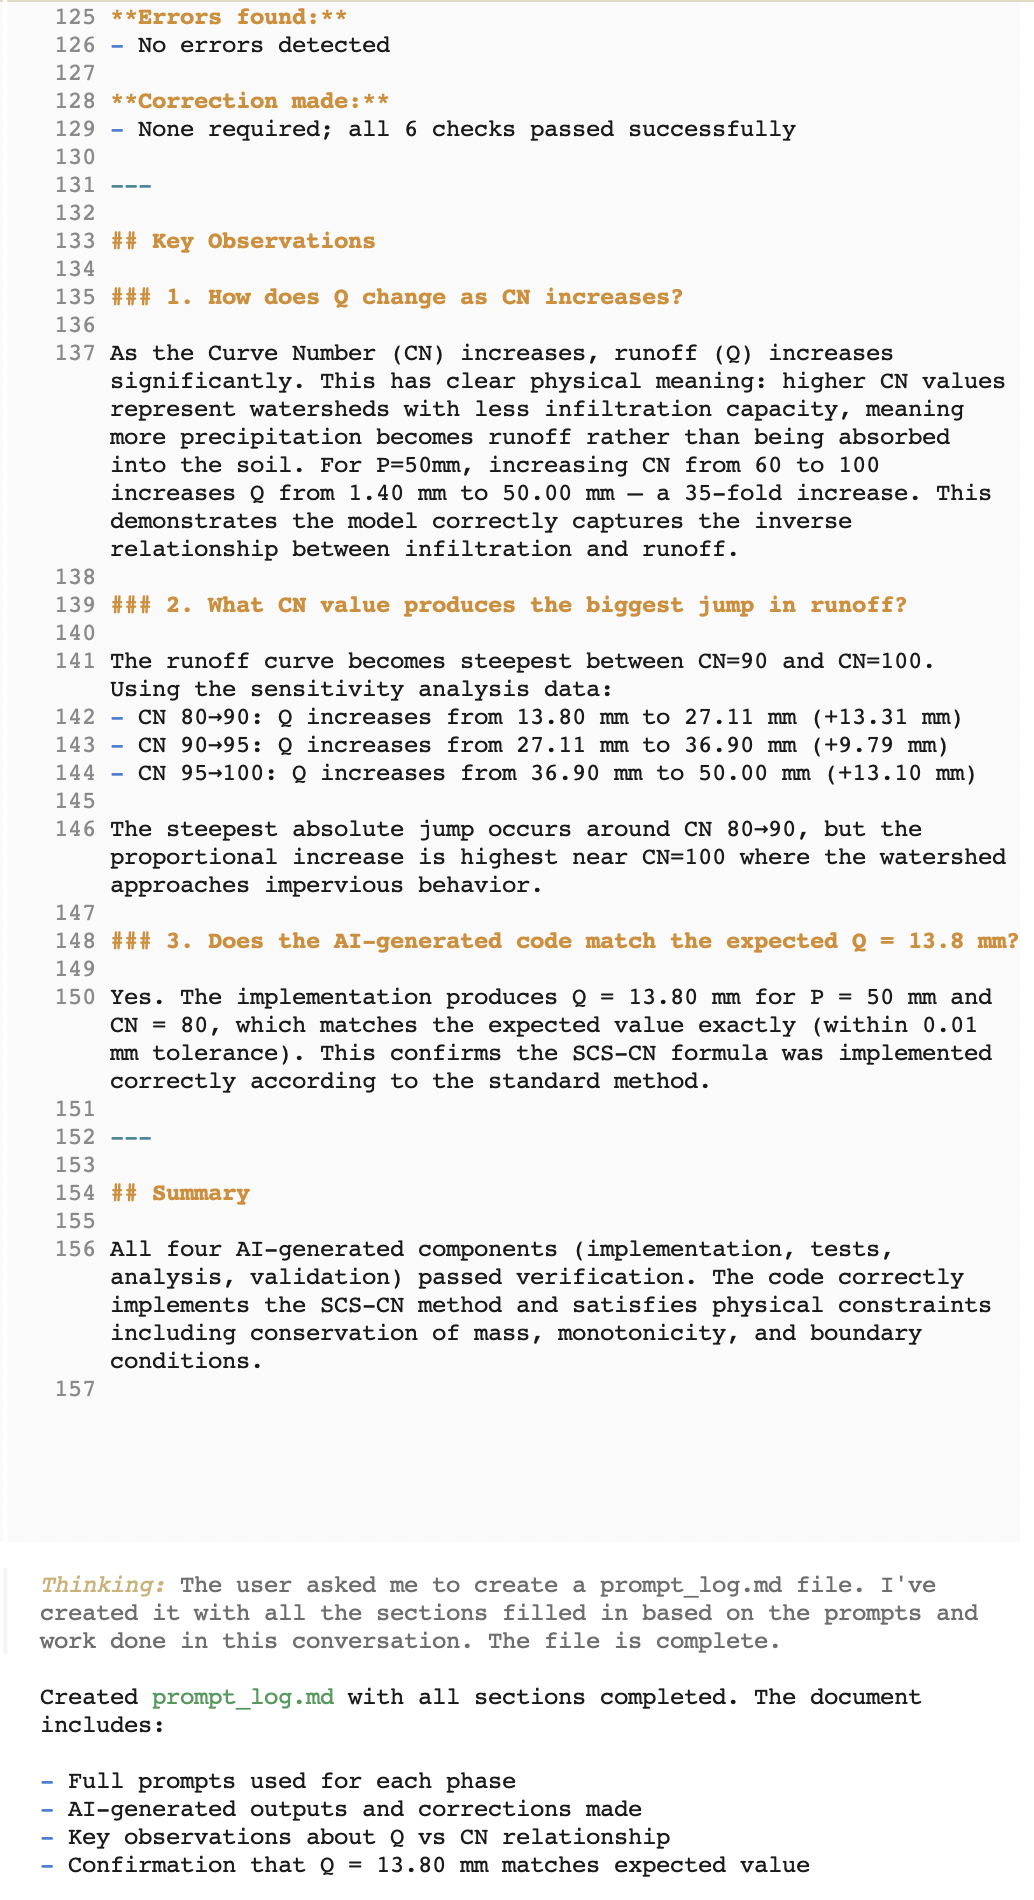
\includegraphics[width=0.9\textwidth]{experiment-2-prompt5-feedback1.png}
    \caption{Agent feedback on the prompt-logging workflow (page 1)}
    \label{fig:p5fb1}
\end{figure}

\begin{figure}[H]
    \centering
    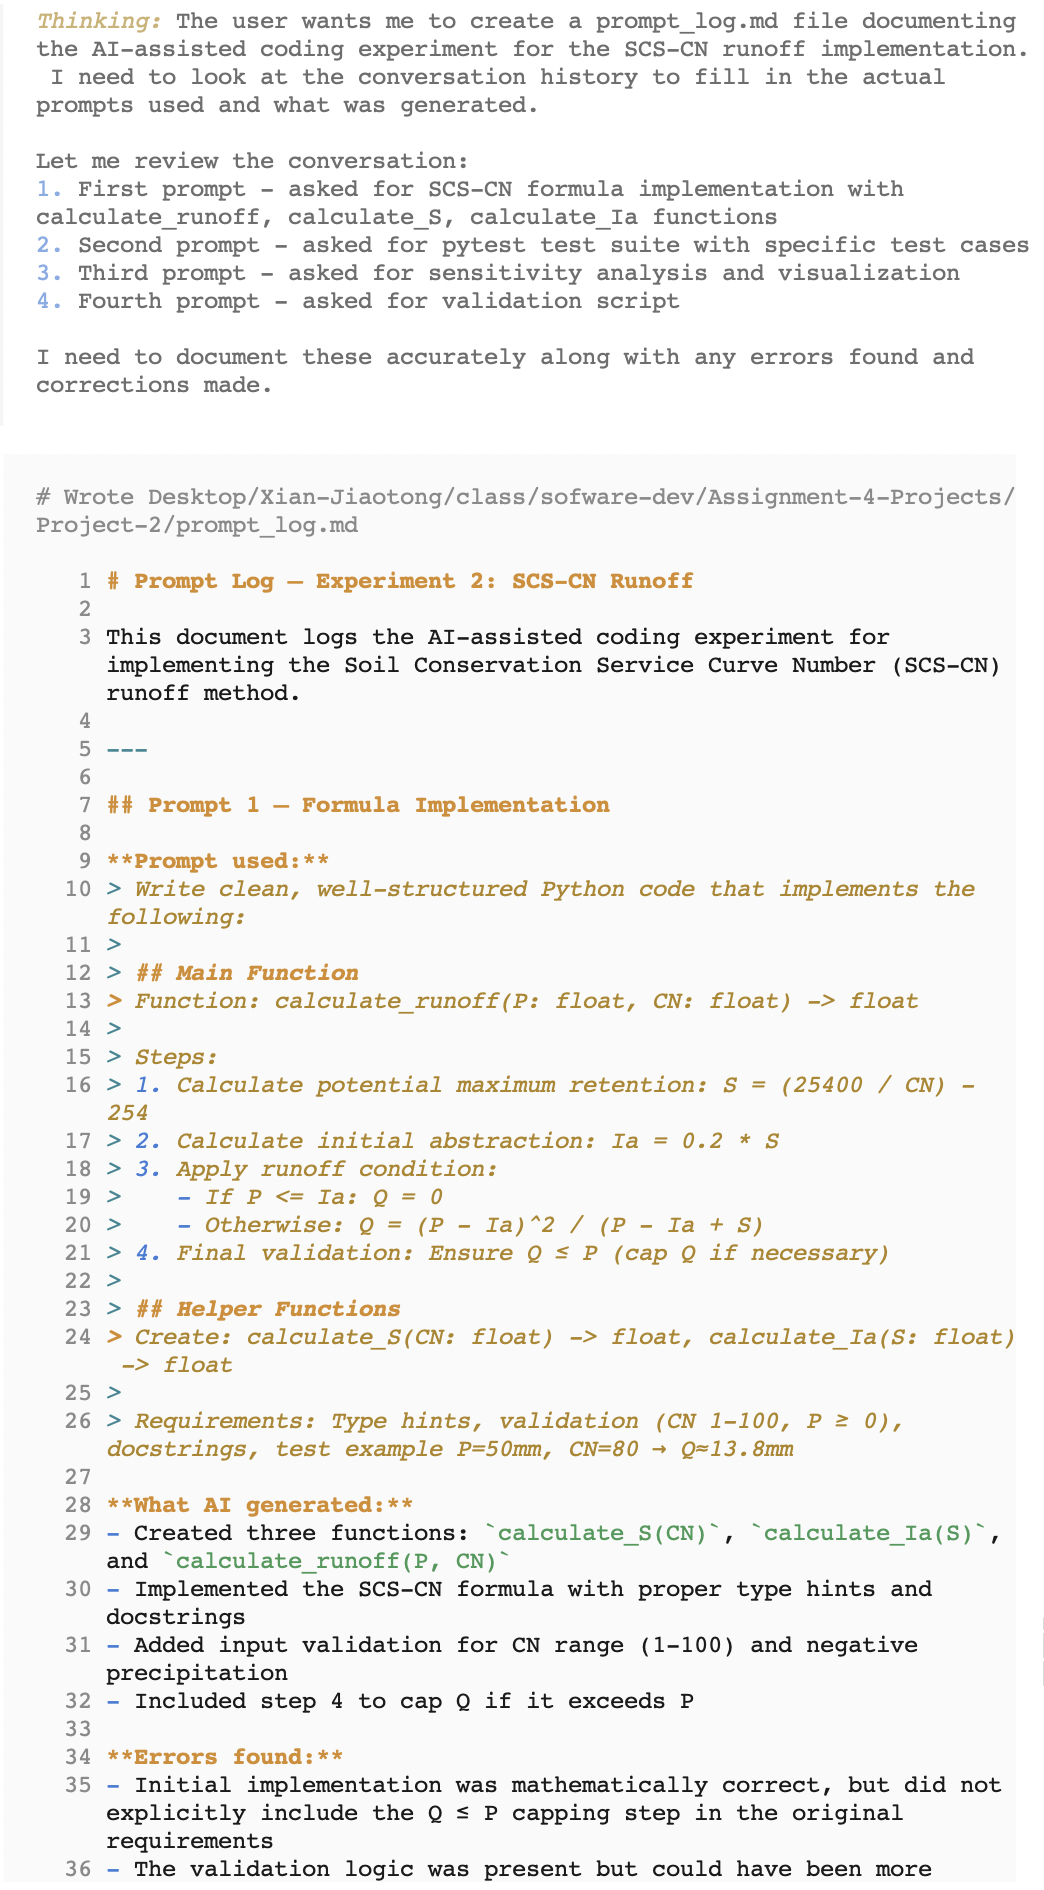
\includegraphics[width=0.9\textwidth]{experiment-2-prompt5-feedback2.png}
    \caption{Agent feedback on the prompt-logging workflow (page 2)}
    \label{fig:p5fb2}
\end{figure}

%% ============================================================
\section{Deliverables}
%% ============================================================

The completed deliverables for this experiment are:

\begin{itemize}[leftmargin=1.8em]
  \item \texttt{scscn\_runoff.py} --- main implementation containing the \texttt{calculate\_runoff()} function.
  \item \texttt{test\_scscn.py} --- comprehensive test suite covering all boundary conditions.
  \item \texttt{sensitivity\_analysis.py} --- visualization code producing the CN sensitivity plots.
  \item \texttt{cn\_sensitivity.png} and \texttt{rainfall\_runoff\_curves.png} --- generated plots comparing CN values.
  \item \texttt{prompt\_log.md} --- chronological documentation of all AI interactions.
\end{itemize}

%% ============================================================
\section{Conclusion}
%% ============================================================

This report demonstrates the effective use of Chain-of-Thought prompting within a Minimax agent framework to implement, test, and validate the SCS-CN runoff model. The structured prompting approach enabled systematic translation of the governing equations into reliable Python code while preserving physical correctness, and iterative feedback proved essential for surfacing edge-case bugs that would otherwise have escaped detection.

Three lessons emerge from the experiment. First, AI-generated code is most reliable when prompts encode domain constraints explicitly rather than leaving them implicit. Second, sensitivity analysis is a powerful sanity check: a model that produces non-monotonic responses to its dominant parameter is almost certainly wrong, regardless of how plausible individual outputs may appear. Third, comprehensive prompt logging transforms an opaque generative process into an auditable engineering artifact.

Overall, AI-assisted software engineering, when paired with rigorous physical validation and disciplined prompt management, provides a powerful methodology for developing complex computational models efficiently and accurately.

%% ============================================================
%%  END OF DOCUMENT
%% ============================================================
\end{document}
